\documentclass{article}
\usepackage[utf8]{inputenc}
\usepackage{geometry}
\usepackage{graphicx}
\usepackage{amsmath}
\usepackage{amsfonts}
\usepackage{amsthm}
\usepackage[most]{tcolorbox}
\usepackage{array}
\usepackage{latexsym}
\usepackage{alltt}
\usepackage{hyperref}
\usepackage{color}
\usepackage{float}
\usepackage{pdfpages}
\usepackage{algorithm}
\usepackage{algpseudocode}
\usepackage{multicol}
\usepackage{multirow}
\usepackage{caption}
\usepackage{xparse}
\usepackage{setspace}
\usepackage{enumitem}


\geometry
{
  a4paper,
  left=15mm,
  right=15mm,
  top=15mm,
  bottom=15mm,
}

% mybox
\newtcolorbox{mybox}[3][]
{
  colframe = #2!25,
  colback  = #2!10,
  coltitle = #2!20!black,  
  title    = {#3},
  #1,
}

\definecolor{my-blue}{cmyk}{0.80, 0.13, 0.14, 0.04, 1.00}

% New environments that use mybox
\newcounter{example}
\newenvironment{example}[1]{\begin{mybox}{green}{\refstepcounter{example}\textbf{Example~\theexample #1}}}{\end{mybox}}

\newenvironment{examplebreak}[1]{\begin{mybox}[breakable]{green}{\refstepcounter{example}\textbf{Example~\theexample #1}}}{\end{mybox}}

\newcounter{definition}
\newenvironment{definition}[1]{\refstepcounter{definition}\begin{mybox}{blue}{\textbf{Definition~\thedefinition #1}}}{\end{mybox}}

\newcounter{theorem}
\newenvironment{theorem}[1]{\begin{mybox}{red}{\refstepcounter{theorem}\textbf{Theorem~\thetheorem #1}}}{\end{mybox}}

\newenvironment{formula}[1]{\begin{mybox}{cyan}{\textbf{#1}}}{\end{mybox}}


% Changing maketitle
\makeatletter         
\renewcommand\maketitle{
{\raggedright % Note the extra {
\begin{center}
{\Large \bfseries \@title}\\[2ex] 
{\large \@author \ - \@date}\\[2ex]
\end{center}}} % Note the extra }
\makeatother

% \onehalfspacing % adjust spacing

% macros
\newcommand{\prob}[1]{\textbf{\textit{P}}\{#1\}}
\NewDocumentCommand{\dsum}{%
    e{^_}
}{%
  {% 
    \displaystyle\sum
    \IfValueT{#1}{^{#1}}
    \IfValueT{#2}{_{#2}}
  }
}%

% maketitle variables
\title{CENG 280 - Chapter 2: Finite Automata}
\author{Burak Metehan Tunçel}
\date{April 2022}

\begin{document}

\maketitle

\section{Deterministic Finite Automata}

\textbf{Finite automaton}, or \textbf{finite-state machine} shares with a real computer the fact that it has a ``central processing unit'' of fixed, finite capacity. It receives its input as a string, delivered to it on an input tape. It delivers no output at all, except an indication of whether or not the input is considered acceptable. It is, in other words, a language recognition device.

What makes the finite automaton such a restricted model of real computers is the \textit{complete absence of memory} outside its fixed central processor.

\begin{figure}[h!]
  \centering
  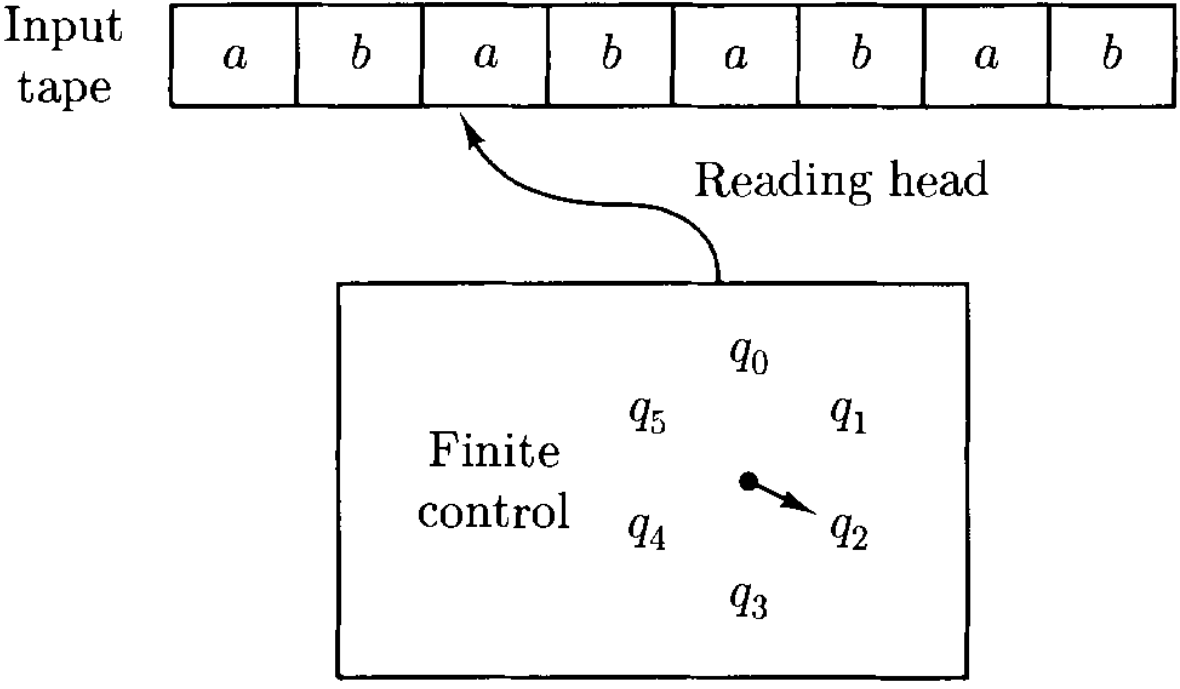
\includegraphics[width=.5\textwidth]{img/Fig2.1.png}
  \caption{Finite Automata}
\end{figure}

\begin{multicols}{2}
\setlength{\columnsep}{1.5cm}
\setlength{\columnseprule}{0.2pt}
  Let's describe the operation of a finite automaton in more detail. 
  \begin{itemize}
    \item Strings are fed into the device by means of an \textbf{input tape}, which is divided into squares, with one symbol inscribed in each tape square (see Figure 1).
    \item The main part of the machine itself is a ``black box'', with innards that can be, at any specified moment, in one of a finite number of distinct internal states.
    \item The black box -called the \textbf{finite control}- can sense what symbol is written at any position on the input tape by means of a movable \textbf{reading head}.
    \item Initially, the reading head is placed at the leftmost square of the tape and the finite control is set in a designated \textbf{initial state}.
    \item At regular intervals the automaton reads one symbol from the input tape and then enters a new state that \textit{depends only on the current state and the symbol just read}.
    \item After reading an input symbol, the reading head moves one square to the right on the input tape so that on the next move it will read the symbol in the next tape square. This process is repeated again and again; a symbol is read, the reading head moves to the right, and the state of the finite control changes. Eventually the reading head reaches the end of the input string.
    \item The automaton then indicates its approval or disapproval of what
    it has read by the state it is in at the end: if it winds up in one of a set of \textbf{final states} the input string is considered to be \textbf{accepted}.
    \item The language accepted by the machine is the set of strings it accepts.
  \end{itemize}
\end{multicols}

\begin{definition}{}
  A \textbf{deterministic finite automaton} is a quintuple $M = (K, \Sigma, \delta, s, F)$ where
  \begin{itemize}
    \item $K$ is a finite set of \textbf{states}
    \item $\Sigma$ is an alphabet,
    \item $s \in K$ is the \textbf{initial state}
    \item $F \subseteq K$ is the set of \textbf{final states}
    \item $\delta$, the \textbf{transition function}, is a function from $K \times \Sigma$ to $K$. 
  \end{itemize}
\end{definition}

The \textbf{configuration} of the machine is the \textit{current state and the unread part of the input string}, i.e., a configuration is an element of $K \times \Sigma^*$.

The binary $\vdash_M$ (yields) relation holds between two configurations of $M$ if and only if the machine can pass from one configuration to another one as a result of a single move. Let $(q, w)$ and $(q',w')$ be two configurations of $M$. Then $(q, w) \vdash_M (q', w')$ if and only if $w = aw'$ for some $a \in \Sigma$ and $q' = \delta(q, a)$. $(q, w) \vdash_M (q', w')$ reads $(q, w)$ \textbf{yields} $(q', w')$ in \textbf{one step}. Note that $\vdash_M$ is a function from $K \times \Sigma^+$ to $K \times \Sigma^*$, hence, for every configuration except $(q, e)$ there exists a uniquely determined next configuration.

$\vdash^*_M$ is the \textbf{reflexive transitive closure} of $\vdash_M$. $(q, w) \vdash^*_M (q', w')$ reads $(q, w)$ \textbf{yields} $(q', w')$. A string $w \in \Sigma^*$ is \textbf{accepted} by $M$ if and only if $(s, w) \vdash^*_M (f, e)$ for some $f \in F$. The \textbf{language} of $M$, $L(M)$, is the set of strings \textit{accepted} by $M$.

\begin{example}{}
  Let $M$ be the deterministic finite automaton $(K, \Sigma, \delta, s, F)$, where
  \begin{multicols}{2}
    \begin{itemize}
      \item $K = \left\{ q_0, q_1 \right\}$
      \item $\Sigma = \left\{ a, b \right\}$
      \item $s = q_0$
      \item $F = \left\{ q_0 \right\}$
    \end{itemize}
  \end{multicols}
  and $\delta$ is the function tabulated below.
  \begin{center}
    \begin{tabular}{c|c|c}
      $q$      & $\sigma$ & $\delta(q, \sigma)$  \\ 
      \hline
      $q_0$ & $a$    & $q_0$             \\
      $q_0$ & $b$    & $q_1$             \\
      $q_1$ & $a$    & $q_1$             \\
      $q_1$ & $b$    & $q_0$            
    \end{tabular}
  \end{center}

  It is then easy to see that $L(M)$ is the set of all strings in $\left\{ a, b \right\}^*$ that have an even number of $b$'s. For $M$ passes from state $q_0$ to $q_1$ or from $q_1$ back to $q_0$ when $a$ $b$ is read, but $M$ essentially ignores $a$'s, always remaining in its current state when an $a$ is read. Thus $M$ counts $b$'s modulo 2, and since $q_0$ (the initial state) is also the sole final state, $M$ accepts a string if and only if the number of $b$'s is even.
  
  If $M$ is given the input $aabba$, its initial configuration is $(q_0, aabba)$. Then 
  \begin{align*}
    (q_0, aabba) &\vdash_M (q_0, abba)\\
    &\vdash_M (q_0, bba)\\
    &\vdash_M (q_1, ba)\\
    &\vdash_M (q_0, a)\\
    &\vdash_M (q_0, e)
  \end{align*}
  Therefore $(q_0, aabba) \vdash^*_M (q_0, e)$, and so $aabba$ is accepted by $M$.
\end{example}

\begin{figure}[h!]
  \centering
  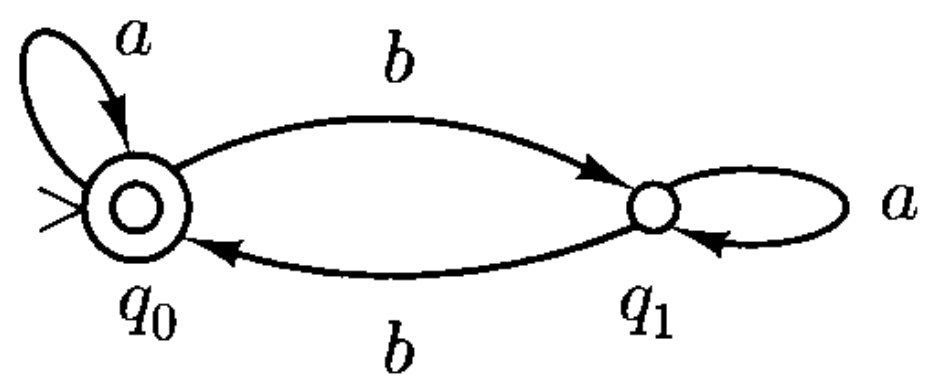
\includegraphics[width=.3\textwidth]{img/Fig2.2.png}
  \caption{State Diagram}
\end{figure}
The tabular representation of the transition function used in this example is not the clearest description of a machine. We generally use a more convenient graphical representation called the \textbf{state diagram} (Figure 2).


\section{Nondeterministic Finite Automata}

In this section we add a powerful and intriguing feature to finite automata.
This feature is called \textbf{nondeterminism}, and is essentially the ability to change states in a way that is only partially determined by the current state and input symbol. That is, we shall now permit several possible ``next states'' for a given combination of current state and input symbol. 

The automaton, as it reads the input string, may choose at each step to go into anyone of these legal next states; the choice is not determined by anything in our model, and is therefore said to be \textit{nondeterministic}. On the other hand, the choice is not wholly unlimited either; only those next states that are legal from a given state with a given input symbol can be chosen. 

\newpage

\begin{figure}[ht!]
  \centering
  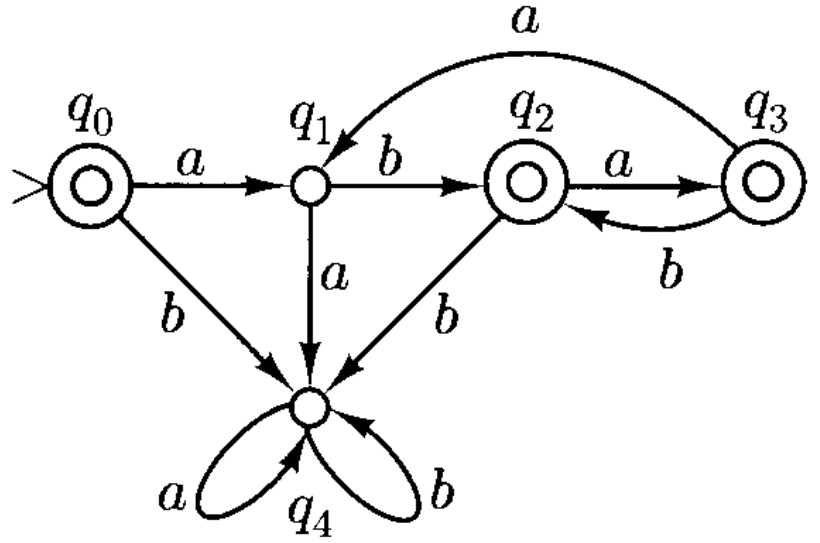
\includegraphics[width=.3\textwidth]{img/Fig2.4.png}
  \caption{}
\end{figure}

To see that a nondeterministic finite automaton can be a much more convenient device to design than a deterministic finite automaton, consider the language $L = (ab \cup aba)^*$, which is accepted by the deterministic finite automaton illustrated in Figure 3.

\begin{figure}[ht!]
  \centering
  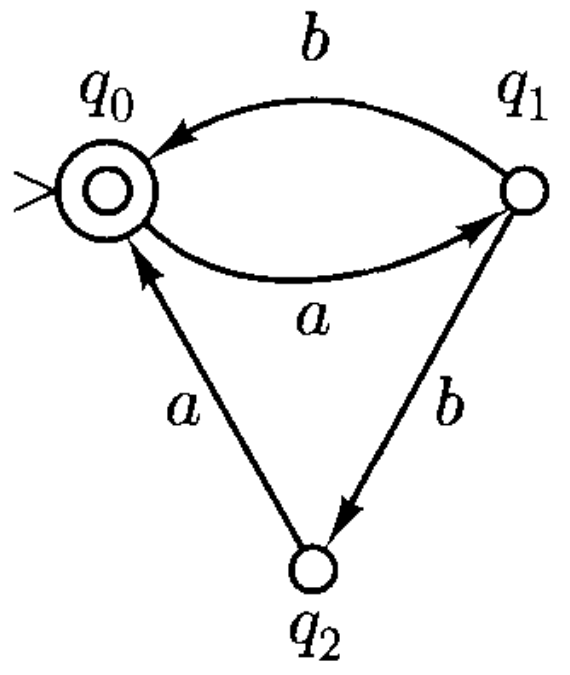
\includegraphics[width=.2\textwidth]{img/Fig2.5.png}
  \caption{}
\end{figure}

$L$ is accepted by the simple nondeterministic device shown in Figure 4. When this device is in state $q_l$ and the input symbol is $b$, there are two possible next states, $q_0$ and $q_2$. Thus Figure 4 does not represent a deterministic finite automaton.

\begin{figure}[ht!]
  \centering
  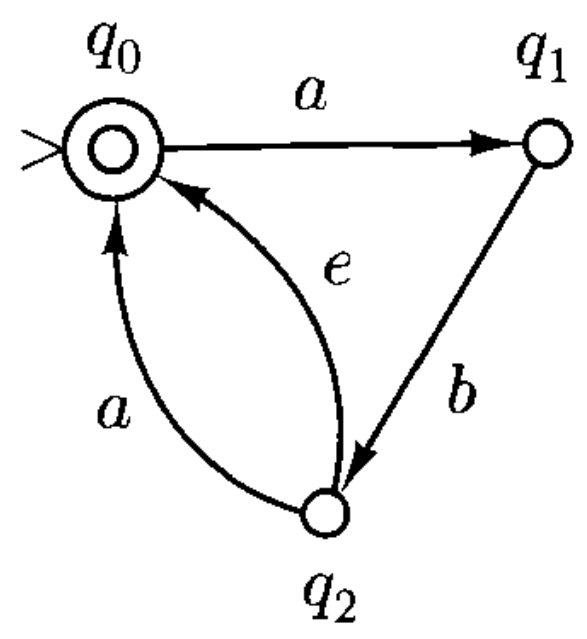
\includegraphics[width=.2\textwidth]{img/Fig2.6.png}
  \caption{}
\end{figure}

We also allow in the state diagram of a nondeterministic automaton arrows that are labeled by the empty string $e$. For example, the device of Figure 5 accepts the same language L. From q2 this machine can return to qo either by reading an $a$ or immediately, without consuming any input.

\begin{definition}{}
  A \textbf{nondeterministic finite automaton} is a quintuple $M = (K, \Sigma, \Delta, s, F)$, where
  \begin{itemize}
    \item $K$ is a finite set of \textbf{states}
    \item $\Sigma$ is an alphabet
    \item $s \in K$ is the \textbf{initial state}
    \item $F \subseteq K$ is the set of \textbf{final states}, and
    \item $\Delta$, the \textbf{transition relation}, is a subset of $K \times (\Sigma \cup \{e\}) \times K$ 
\end{itemize}
\end{definition}

$(q, a, p) \in \Delta$ is called a \textbf{transition} of $M$. $(q, e, p)$ indicates that the machine can pass to state $p$ from state $q$ without reading an input symbol.

\newpage
\begin{multicols}{2}
\setlength{\columnsep}{1.5cm}
\setlength{\columnseprule}{0.2pt}
  The configuration of the machine is the current state and the unread part of the input string, i.e., a configuration is an element of $K \times \Sigma^*$.\\

  The binary $\vdash_M$ (\textbf{yields}) relation holds between two configurations of $M$ if and only if the machine can pass from one configuration to another one as a result of a \textit{single move}. Let $(q, w)$ and $(q', w')$ be two configurations of $M$. Then $(q, w) \vdash_M (q', w')$ if and only if $w = aw'$ for some $a \in \Sigma \cup \{e\}$ and $(q, a, q') \in \Delta$. $(q, w) \vdash_M (q', w')$ reads $(q, w)$ \textbf{yields} $(q', w')$ \textbf{in one step}. Note that $\vdash_M$ might not be a function, i.e., there might be several pairs $(q', w')$ (or none at all) such that $(q, w) \vdash_M (q', w')$.\\

  $\vdash^*_M$ is the \textbf{reflexive transitive closure} of $\vdash_M$. $(q, w) \vdash^*_M (q', w')$ reads $(q, w)$ yields $(q', w')$. A string $w \in \Sigma^*$ is \textbf{accepted} by $M$ if and only if there is a state $f \in F$ such that $(s, w) \vdash^*_M (f, e)$. The \textbf{language} of $M$, $L(M)$, is the set of strings accepted by $M$.\\

  A deterministic finite state automaton is just a special type of nondeterministic finite state automaton. We obtain a DFA when $\Delta$ defines a function from $K \times \Sigma$ to $K$. In other words, an NFA $M = (K, \Sigma, \Delta, s, F)$ is deterministic if there are no transitions of the form $(q, e, p)$ and for each $q \in K$ and $a \in \Sigma$, there exists \textit{exactly one} $p \in K$ such that $(q, a, p) \in \Delta$.\\

  We can conclude that the class of languages recognized by deterministic finite state automaton is a \textit{subset} of the class of languages recognized by nondeterministic finite state automaton. Essentially, these classes are the same: A nondeterministic finite automaton can always be
  converted to an \textit{equivalent} deterministic finite state automaton.\\

  Two automaton $M_1$ and $M_2$ are said to be \textbf{equivalent} when $L(M_1) = L(M_2)$.
\end{multicols}

\begin{theorem}{}
  \textit{For each nondeterministic finite automaton, there exists an equivalent deterministic finite automaton.}
\end{theorem}

\begin{proof}
  The proof of the theorem is constructive: use \textbf{subset construction} algorithm to construct a DFA from an NFA and then show they are equivalent. Given an NFA $M = (K, \Sigma, \Delta, s, F)$, the algorithm constructs an equivalent DFA $M' = (K', \Sigma, \delta, s', F')$ as follows. For each state $q \in K$, the set of states that can be reached without reading an input symbol is defined as
  \begin{align*}
    E(q) = \left\{ p \in K\ |\ (q, e) \vdash^*_M (p, e) \right\}& &\textnormal{(Check Example 2)}
  \end{align*}
  Essentially, $E(q)$ is the reflexive transitive closure of the set $\left\{ q \right\}$ under the relation $\left\{(p, r)\ |\ (p, e, r) \in \Delta \right\}$. The DFA is defined as:
  \begin{align*}
    K' &= 2^K\\
    s' &= E(s)\\
    F' &= \left\{ Q \subseteq K\ |\ Q \cap F \neq \emptyset \right\}\\
    \delta'(Q, a) &= \left\{ E(p) : p \in K, (q, a, p) \in \Delta \textnormal{ for some } q \in Q \right\} \textnormal{ for each $Q \in K'$ and $a \in \Sigma$}\\
    &= \bigcup \left\{ E(p) : p \in K, (q, a, p) \in \Delta \textnormal{ for some } q \in Q \right\}
  \end{align*}
  To prove that $M$ and $M'$ are equivalent, show that for any string $w \in \Sigma^*$
  \begin{equation*}
    (s, w) \vdash^*_M (f, e) \textnormal{ for some } f \in F \textnormal{ iff } (E(s), q) \vdash^*_{M'} (P, e) \textnormal{ for some } P \in F'
  \end{equation*}
  Thus they recognize the same language.
\end{proof}

\begin{figure}[ht!]
  \centering
  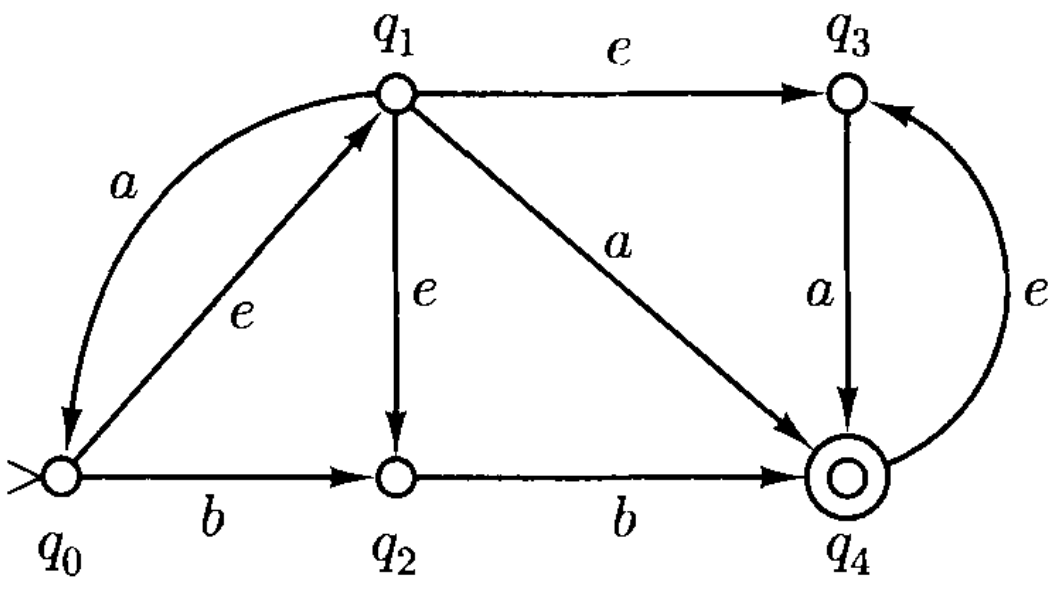
\includegraphics[width=.3\textwidth]{img/Fig2.9.png}
  \caption{}
\end{figure}

\begin{examplebreak}{}
  In the automaton of Figure 6, we have $E(q_0) = \left\{ q_0, q_1, q_2, q_3  \right\}$, $E(q_1) = \left\{ {q_1, q_2, q_3} \right\}$, $E(q_2) = \left\{ q_2 \right\}$, $E(q_3) = \left\{ q_3 \right\}$, and $E(q_4) = \left\{ q_3, q_4 \right\}$.
\end{examplebreak}


\begin{figure}[t]
  \centering
  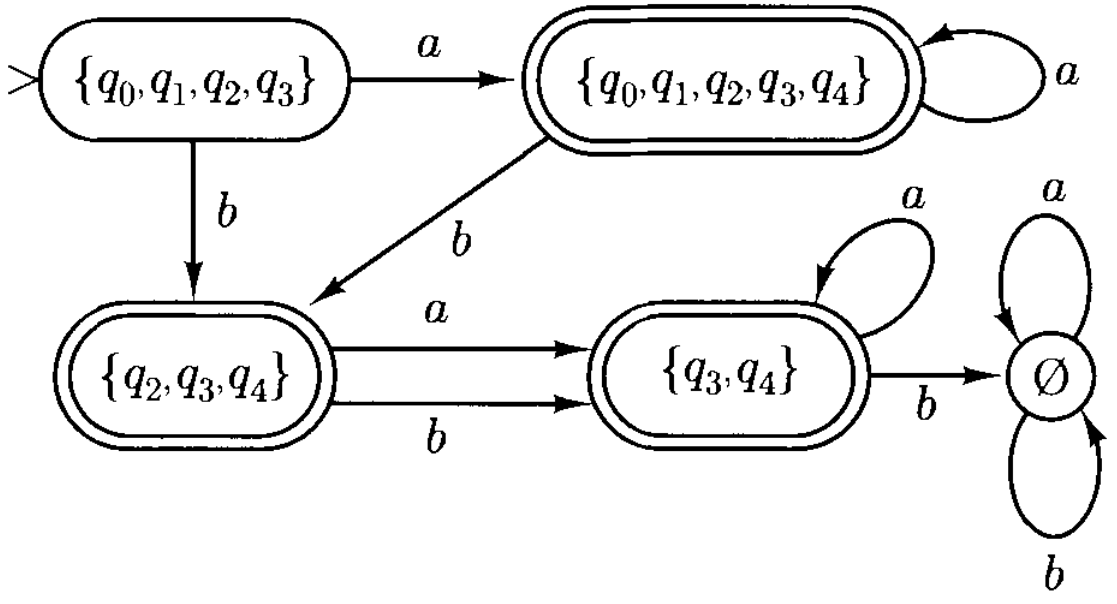
\includegraphics[width=.5\textwidth]{img/Fig2.10.png}
  \caption{}
\end{figure}


\begin{examplebreak}{: NFA to DFA}
  \quad Let's apply the algorithm then to the nondeterministic automaton in Figure 6. Since $M$ has 5 states, $M'$ will have $2^5 = 32$ states. However, only a few of these states will be relevant to the operation of $M'$ -namely, those states that can be reached from state $s'$ by reading some input string. Obviously, any state in $K'$ that is not reachable from $s'$ is irrelevant to the operation of $M'$ and to the language accepted by it. We shall build this reachable part of $M'$ by starting from $s'$ and introducing a new state only when it is needed as the value of $\delta'(q, a)$ for some state $q \in K'$ already introduced and some $a \in \Sigma$.
  
  \quad We have already defined $E(q)$ for each state $q$ of $M$ (from Example 2). Since $s' = E(q_0) = \left\{ q_0, q_1, q_2, q_3  \right\}$,
  \begin{equation*}
    (q_1, a, q_0),\ (q_1, a, q_4), \textnormal{ and } (q_3, a, q_4)
  \end{equation*}
  are all the transitions $(q, a, p)$ for some $q \in s'$. It follows that
  \begin{equation*}
    \delta'(s', a) = E(q_0) \cup E(q_4) = \left\{ q_0, q_1, q_2, q_3, q_4 \right\}
  \end{equation*}
  Similarly,
  \begin{equation*}
    (q_0, b, q_2) \textnormal{ and } (q_2, b, q_4)
  \end{equation*}
  are all the transitions of the form $(q, b, p)$ for some $q \in s'$, so
  \begin{equation*}
    \delta'(s', b) = E(q_2) \cup E(q_4) = \left\{ q_2, q_3, q_4 \right\}
  \end{equation*}
  Repeating this calculation for the newly introduced states, we have the following,,
  \begin{align*}
    \delta'(\left\{ q_0, q_1, q_2, q_3, q_4 \right\}, a) &= \left\{ q_0, q_1, q_2, q_3, q_4 \right\}\\
    \delta'(\left\{ q_0, q_1, q_2, q_3, q_4 \right\}, b) &= \left\{ q_2, q_3, q_4 \right\}\\
    \delta'(\left\{ q_2,q_3,q_4 \right\},a) &= E(q_4) = \left\{ q_3,q_4 \right\}\\
    \delta'(\left\{ q_2,q_3,q_4 \right\},b) &= E(q_4) = \left\{ q_3,q_4 \right\}
  \end{align*}
  Next,
  \begin{align*}
    \delta'(\left\{ q_3, q_4 \right\}, a) &= E(q_4) = \left\{ q_3, q_4 \right\}\\
    \delta'(\left\{ q_3, q_4 \right\}, b) &= 0
  \end{align*}
  and finally
  \begin{equation*}
    \delta'(\emptyset, a) = \delta'(\emptyset, b) = \emptyset
  \end{equation*}
  The relevant part of $M'$ is illustrated in Figure 7. $F'$, the set of final states, contains each set of states of which $q_4$ is a member, since $q_4$ is the sole member of $F$; so in the illustration, the three states $\left\{ q_0, q_1, q_2, q_3, q_4 \right\}$, $\left\{ q_2, q_3, q_4 \right\}$, and $\left\{ q_3,q_4 \right\}$ of $M'$ are final.
\end{examplebreak}

\textit{Basically, first look the initial state of NFA. E(s), a set, will be the initial state of DFA. It was $\left\{ q_0, q_1, q_2, q_3 \right\}$ for the example 3. Then look the each element of the set, if there is a way to any other state by reading an input inside alphabet (in example it is (a, b)), note that state(s) and combine their E(s'). In the first part of example $\delta'(s', a) = E(q_0) \cup E(q_4) = \left\{ q_0, q_1, q_2, q_3, q_4 \right\}$. When introduce new state, repeat that.}


\section{Finite Automata and Regular Expressions}

The main result of the last section was that the class of languages accepted by finite automata remains the same even if a new and seemingly powerful feature -\textit{nondeterminism}- is allowed. This suggests that the class of languages accepted by finite automata has a sort of \textit{stability}: Two different approaches, one apparently more powerful than the other, end up defining the same class. In this section we shall prove another important characterization of this class of languages, further evidence of how remarkably stable it is: The class of languages accepted by finite automata, deterministic or nondeterministic, is the same as the class of \textit{regular languages} -those that can be described by regular expressions.

\begin{theorem}{}
  The class of languages accepted by finite automata is closed under 
  \begin{enumerate}[label=\alph*)]
    \item union
    \item concatenation
    \item Kleene star
    \item complementation
    \item intersection
  \end{enumerate}
\end{theorem}

\begin{proof}
  In each case we show how to construct an automaton $M$ that accepts the appropriate language, given two automata $M_1$ and $M_2$ (only $M_1$ in the cases of Kleene star and complementation).

  \begin{enumerate}[label=(\alph*)]
    % (a) Union
    \item \textit{Union.}
    Let $M_1 = (K_1, \Sigma, \Delta_1, s_1, F_1)$ and $M_2 = (K_2, \Sigma, \Delta_2, s_2, F_2)$ be nondeterministic finite automata; we shall construct a nondeterministic finite automaton $M$ such that $L(M) = L(M_1) \cup L(M_2)$. The construction of $M$ is rather simple and intuitively clear, illustrated in Figure 8. Basically, $M$ uses nondeterminism to guess whether the input is in $L(M_1)$ or in $L(M_2)$, and then processes the string exactly as the corresponding automaton would; it follows that $L(M) = L(M_1) \cup L(M_2)$. But let us give the formal details and proof for this case.
    \begin{figure}[h!]
      \centering
      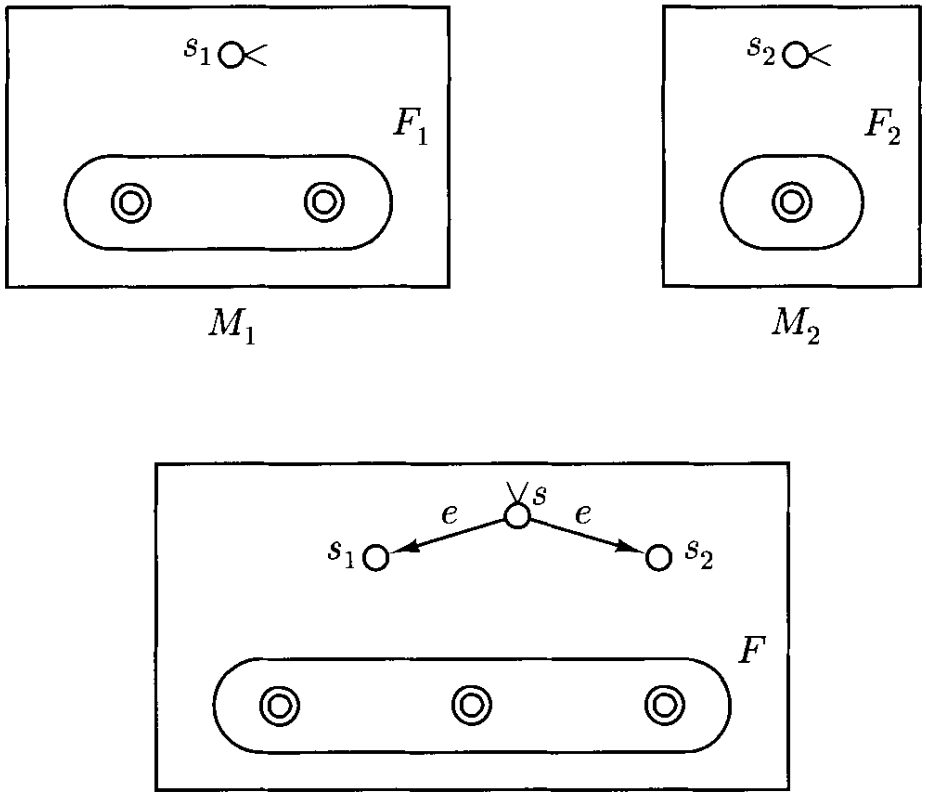
\includegraphics[width=.5\textwidth]{img/Fig2.11.png}
      \caption{}
    \end{figure}
    Without loss of generality, we may assume that $K_1$ and $K_2$ are disjoint sets. Then the finite automaton $M$ that accepts $L(M_1) \cup L(M_2)$ is defined as follows
    
    \quad $M = (K, \Sigma, \Delta, s, F)$, where $s$ is a new state not in $K_1$ or $K_2$,
    \begin{itemize}
      \item $K = K_1 \cup K_2 \cup \left\{ s \right\}$
      \item $F = F_1 \cup F_2$
      \item $\Delta = \Delta_1 \cup \Delta_2 \cup \left\{ (s,e,s_1),(s,e,s_2) \right\}$
    \end{itemize}
    That is, $M$ begins any computation by nondeterministically choosing to enter either the initial state of $M_1$ or the initial state of $M_2$ ,and thereafter, $M$ imitates either $M_1$ or $M_2$. Formally, if $w \in \Sigma^*$, then $(s, w) \vdash^*_M (q, e)$ for some $q \in F$ if and only if either $(s_1, w) \vdash^*_{M_1} (q, e)$ for some $q \in F_2$, or $(s_2, w) \vdash^*_{M_2} (q, e)$ for some $q \in F_2$. Hence $M$ accepts $w$ if and only if $M_1$ accepts $w$ or $M_2$ accepts $w$, and $L(M) = L(M_1) \cup L(M_2)$.

    % (b) Concatenation
    \item \textit{Concatenation.}
    Again, let $M_1$ and $M_2$ be nondeterministic finite automata; we construct a nondeterministic finite automaton $M$ such that $L(M) = L(M_1) L(M_2)$. The construction is shown schematically in Figure 9; $M$ now operates by simulating $M_1$ for a while, and then ``\textit{jumping}'' nondeterministically from a final state of $M_1$ to the initial state of $M_2$. Thereafter, $M$ imitates $M_2$. 

    \begin{figure}[h!]
      \centering
      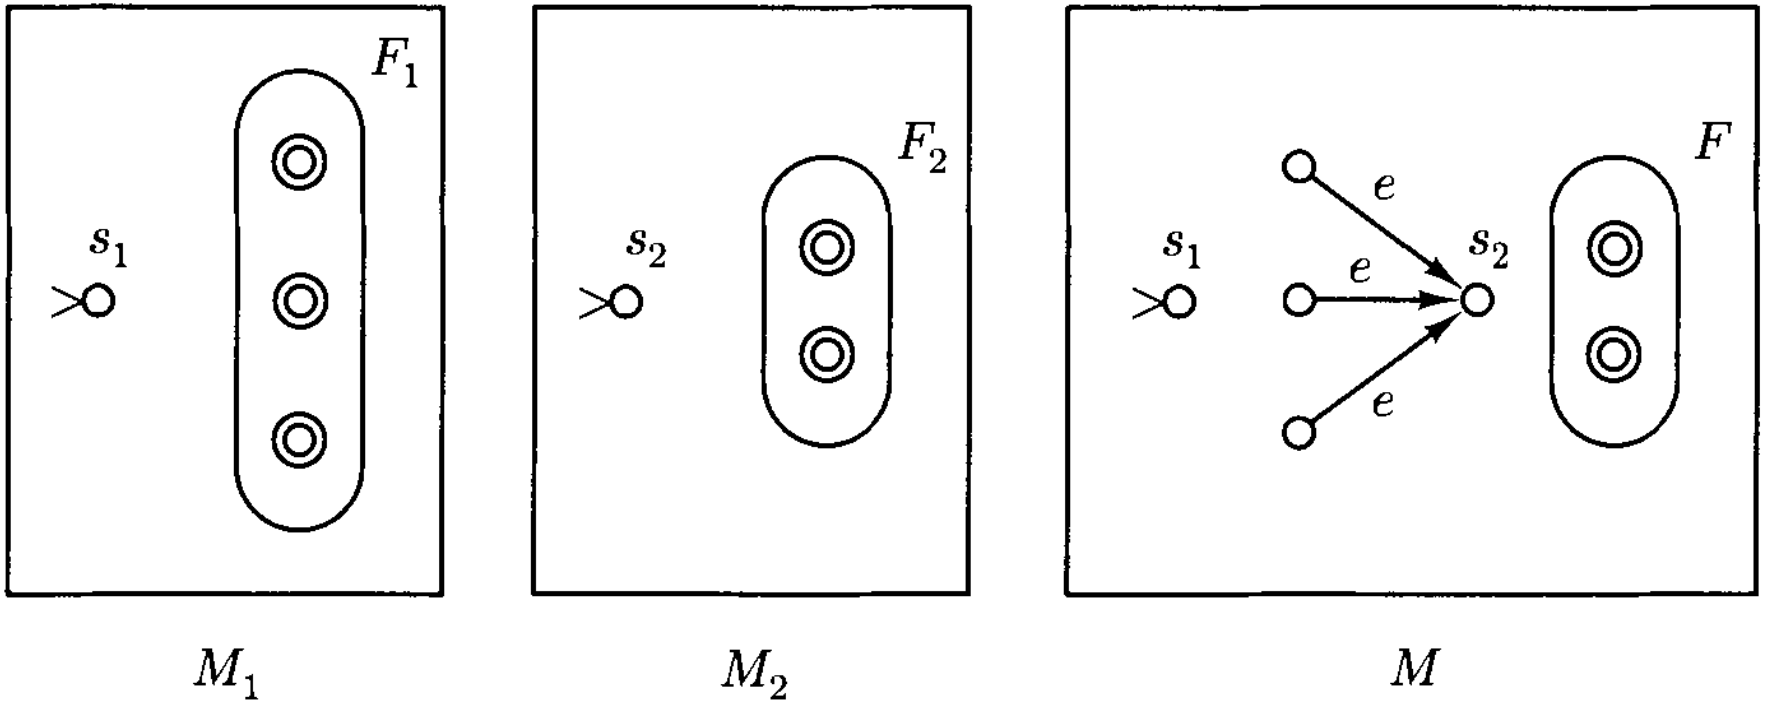
\includegraphics[width=.5\textwidth]{img/Fig2.12.png}
      \caption{}
    \end{figure}

    Then the finite automaton $M$ that accepts $L(M_1) L(M_2)$ is defined as follows (\textit{May include mistakes})
    
    \quad $M = (K, \Sigma, \Delta, s, F)$
    \begin{itemize}
      \item $s = s_1$
      \item $K = K_1 \cup K_2$
      \item $F = F_2$
      \item $\Delta = \Delta_1 \cup \Delta_2 \cup \left\{ (f,e,s_2)\ |\ f \in F_1 \right\}$
    \end{itemize}

    % (c) Kleenestar
    \item \textit{Kleene star.}
    Let $M_1$ be a nondeterministic finite automaton; we construct a nondeterministic finite automaton $M$ such that $L(M) = L(M_1)^*$. The construction is similar to that for concatenation, and is illustrated in Figure 10. $M$ consists of the states of $M_1$ and all the transitions of $M_1$; any final state of $M_1$ is a final state of $M$. In addition, $M$ has a new initial state $s$. This new initial state is also final, so that $e$ is accepted. From $s$ there is an $e$-transition to the initial state $s_1$ of $M_1$, so that the operation of $M_1$ can be initiated after $M$ has been started in state $s$. Finally, $e$-transitions are added from each final state of $M_1$ back to $s_1$; this way, once a string in $L(M_1)$ has been read, computation can resume from the initial state of $M_1$.

    \begin{figure}[h!]
      \centering
      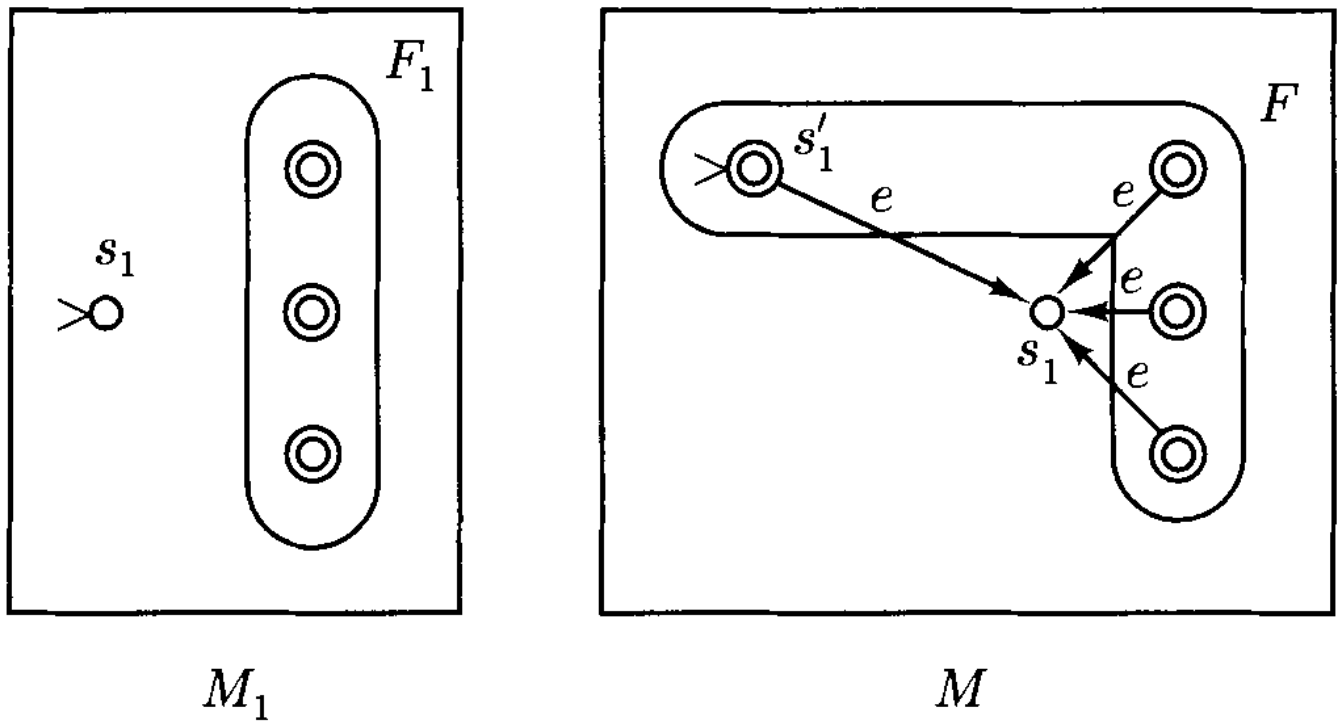
\includegraphics[width=.40\textwidth]{img/Fig2.13.png}
      \caption{}
    \end{figure}

    Then the finite automaton $M$ that accepts $L(M_1)^*$ is defined as follows (\textit{May include mistakes})

    \quad $M = (K, \Sigma, \Delta, s, F)$, where $s$ is not in $M_1$
    \begin{itemize}
      \item $K = K_1 \cup \left\{ s \right\}$
      \item $F = F_1 \cup \left\{ s \right\}$
      \item $\Delta = \Delta_1 \cup \left\{ (s,e,s_1) \right\}$
    \end{itemize}

    % (d) Complementation
    \item \textit{Complementation.}
    Let $M = (K, \Sigma, \delta, s, F)$ be a \textit{deterministic} finite automaton. Then the complementary language $\overline{L} = \Sigma^* - L(M)$ is accepted by the deterministic finite automaton $M = (K, \Sigma, \delta, s, K - F)$. That is, $\overline{M}$ is identical to $M$ except that final and non final states are interchanged.

    Then the finite automaton $M$ that accepts $\overline{L(M_1)}$ is defined as follows (\textit{May include mistakes})

    \quad $M = (K, \Sigma, \Delta, s, F)$.
    \begin{itemize}
      \item $s = s_1$
      \item $K = K_1$
      \item $F = K \setminus F_1$
      \item $\Delta = \Delta_1$
    \end{itemize}

    % (e) Intersection
    \item \textit{Intersection.}
    Just recall that
    \begin{equation*}
      L_1 \cap L_2 = \Sigma^* - \left( \left( \Sigma^* - L_1 \right) \cup \left( \Sigma^* - L_2 \right) \right)
    \end{equation*}
    and so closedness under intersection follows from closedness under union and complementation ((a) and (d) above). So, basically
    \begin{equation*}
      L(M) = L(M_1) \cap L(M_2) = \overline{\overline{L(M_1)} \cup \overline{L(M_2)}}
    \end{equation*}
  \end{enumerate}
\end{proof}

\begin{theorem}{}
  \textit{A language is regular if and only if it is accepted by a finite automaton.}
\end{theorem}

\begin{proof}
  \begin{itemize}
    \item \textit{Only if}. Recall that the class of regular languages is the smallest class of languages containing the empty set $\emptyset$ and the singletons $a$, where $a$ is a symbol, and \textit{closed under union, concatenation, and Kleene star}.

    It is evident (see Figure 11) that the empty set and all singletons are indeed accepted by finite automata; and by Theorem 2 the finite automaton languages are closed under \textit{union}, \textit{concatenation}, and \textit{Kleene star}. Hence \textit{every regular language is accepted by some finite automaton}.

    \begin{example}{}
      Consider the regular expression $(ab \cup aab)^*$. A nondeterministic finite automaton accepting the language denoted by this regular expression can be built up using the methods in the proof of the various parts of Theorem 2, as illustrated in Figure 11.
    \end{example}

    \begin{figure}[h!]
      \centering
      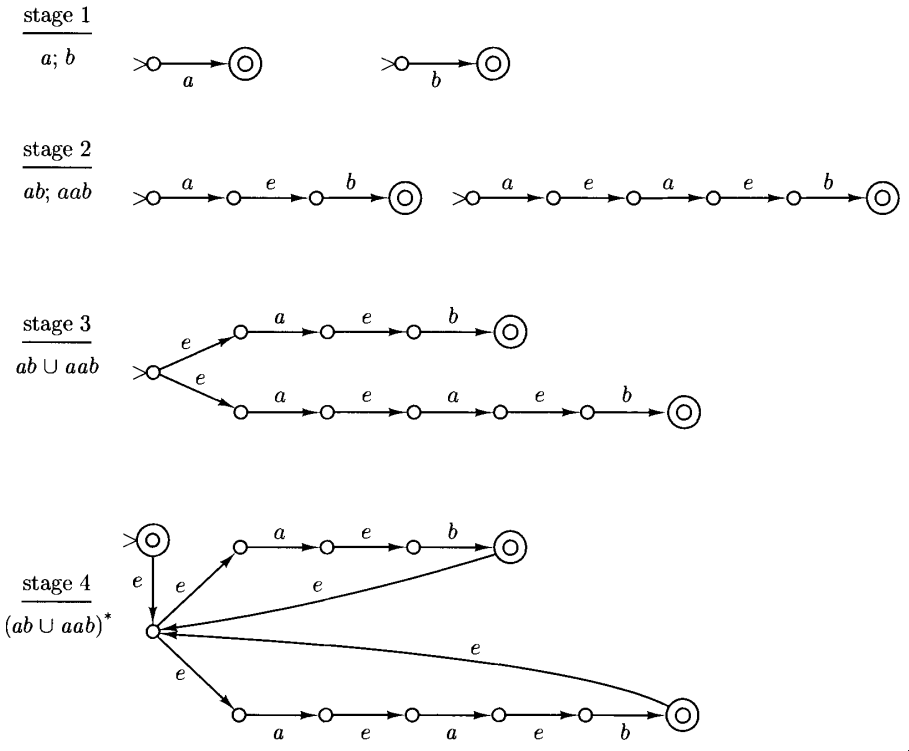
\includegraphics[width=.95\textwidth]{img/Fig2.14.png}
      \caption{}
    \end{figure}

    
    \item \textit{If}. Let $M = (K, \Sigma, \Delta, s, F)$ be a finite automaton (not necessarily deterministic). We shall construct a regular expression $R$ such that $L(R) = L(M)$. We shall represent $L(M)$ as the union of many (but a finite number of) simple languages. Let $K = \left\{ q_1, ..., q_n  \right\}$ and $s = q_1$. For $i, j = 1, ..., n$ and $k = 0, ..., n$:
    \begin{quote}
      $R(i, j, k)$: the set of strings $w \in \Sigma^*$ that can be read by $M$ starting from $q_i$ to $q_j$ without passing through an intermediate state from $\left\{ q_{k+1}, ..., q_n \right\}$ -the endpoints $q_i$ and $q_j$ are allowed to be numbered higher than $k$.
    \end{quote}
    That is, $R(i, j, k)$ is the set of strings spelled by all paths from $q_i$ to $q_j$ of rank $k$ (recall the similar maneuver in the computation of the reflexive-transitive closure of a relation, in which we again considered paths with progressively higher and higher-numbered intermediate nodes). When $k = n$, it follows that
    \begin{equation*}
      R(i,j,n) = \left\{ w \in \Sigma^*\ |\ (q_i, w) \vdash^*_M (q_j, e) \right\}
    \end{equation*}
    Therefore,
    \begin{equation*}
      L(M) = \bigcup \left\{ R(1, j, n)\ |\ q_j \in F \right\}
    \end{equation*}
    The crucial point is that all of these sets $R(i, j, k)$ are regular, and hence so is $L(M)$.

    \quad The proof that each $R(i, j, k)$ is regular is by induction on $k$. For $k = 0$, $R(i, j, 0)$:
    \begin{itemize}
      \item $\left\{ a \in \Sigma \cup \left\{ e \right\}\ |\ (q_i, a, q_j) \in \Delta \right\}$ if $i\neq j$
      \item $\left\{ e \right\} \cup \left\{ a \in \Sigma \cup \left\{ e \right\}\ |\ (q_i, a, q_j) \in \Delta \right\}$ if $i = j$.
    \end{itemize}
    $R(i, j, 0)$ is either singleton or empty for each $i$, $j$, hence regular.

    \quad For the induction step, suppose that $R(i, j, k-1)$ for all $i$, $j$ have been defined as regular languages for all $i$, $j$. Then each set $R(i, j, k)$ can be defined combining previously defined regular languages by the regular operations of union, Kleene star, and concatenation, as follows:
    \begin{equation*}
      R(i, j, k) = R(i, j, k - 1) \cup R(i, k, k - 1) R(k, k, k - 1)^* R(k, j, k - 1)
    \end{equation*}
    This equation states that to get from $q_i$ to $q_j$ without passing through a state numbered greater than $k$, $M$ may either
    \begin{enumerate}
      \item go from $q_i$ to $q_j$ without passing through a state numbered greater than $k - 1$; or
      \item go (a) from $q_i$ to $q_k$; then (b) from $q_k$ to $q_k$ zero or more times; then (c) from $q_k$ to $q_j$; in each case without passing through any intermediate states numbered greater than $k - 1$
    \end{enumerate}
    Consequently, if $R(i, j, k - 1)$ is regular for each $i$, $j$, then $R(i, j, k)$ is also regular for all $i$, $j$, $k$. By induction, $R(i, j, n)$ is regular.
  \end{itemize}
\end{proof}

The proof of the theorem is used to generate a regular expression from a finite state automaton. Its application is simpler when the automaton is in the following special form
\begin{itemize}
  \item the automaton has a single final state, $F = \{f\}$
  \item the initial state does not have an incoming transition
  \item the final state does not have an outgoing transition
\end{itemize}

\noindent Every automaton can be converted to an equivalent automaton in special form.

\quad RE construction from FA:
\begin{enumerate}
  \item Convert FA to an NFA in special form.
  \item For each $k = 0, ..., n$, and for each $i, j = 1, ..., n$: Compute $R(i, j, k)$
  \item Return $R(s, f, n)$
\end{enumerate}


\begin{figure}[t]
  \centering
  \begin{minipage}{.35\textwidth}
    \centering
    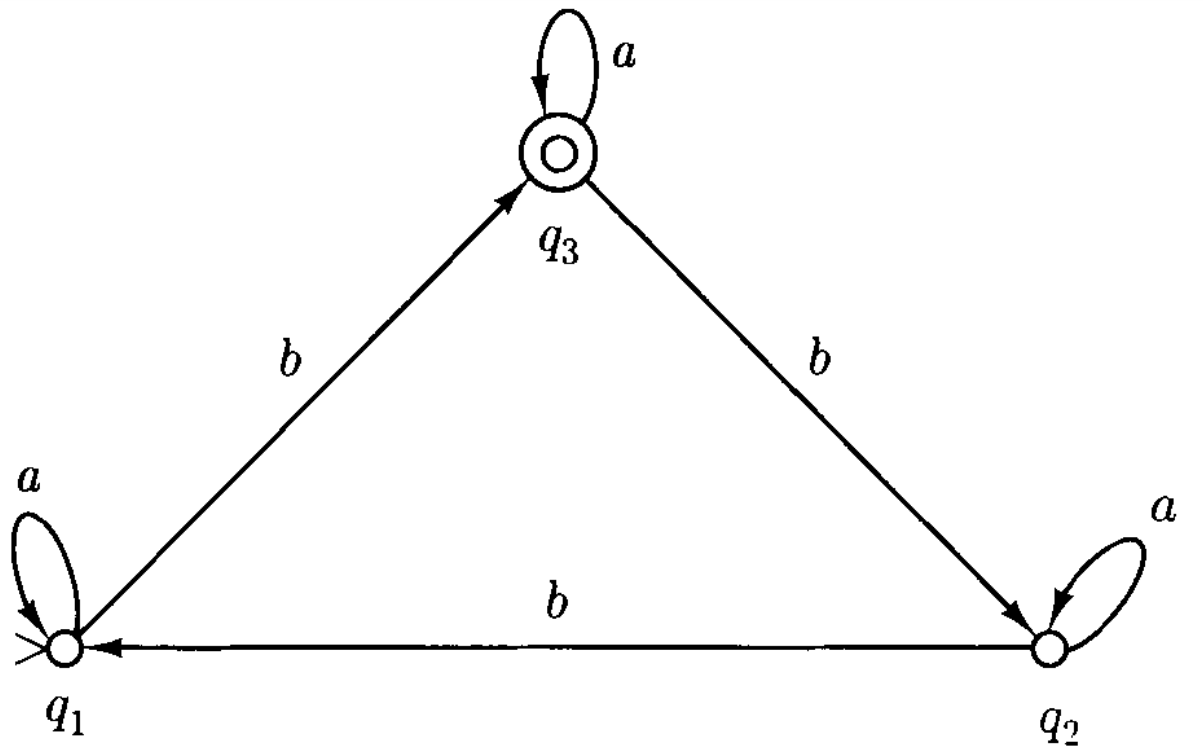
\includegraphics[width=\textwidth]{img/Fig2.15.png}
    \caption{}
  \end{minipage}
  \begin{minipage}{.43\textwidth}
    \centering
    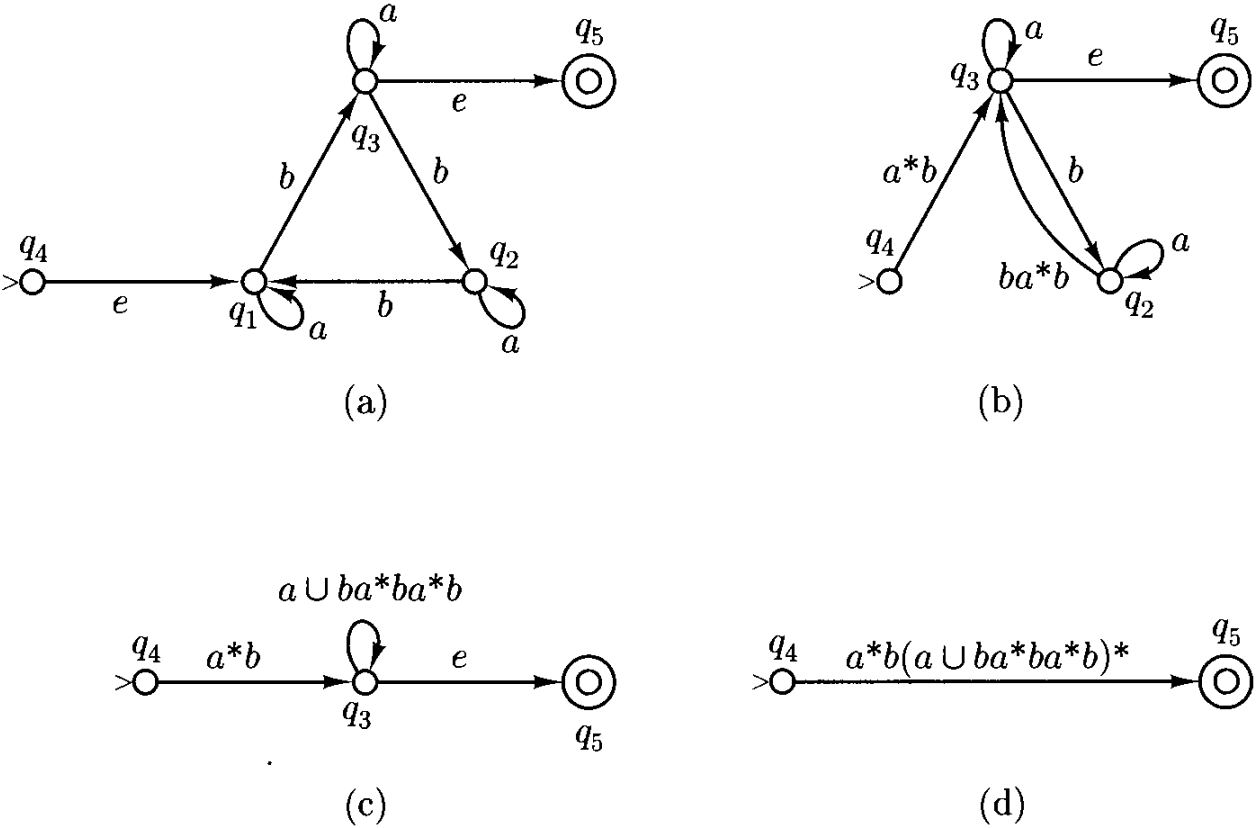
\includegraphics[width=\textwidth]{img/Fig2.16.png}
    \caption{}
  \end{minipage}
\end{figure}

\begin{examplebreak}{}
  Let us construct a regular expression for the language accepted by the deterministic finite automaton of Figure 12. This automaton accepts the language
  \begin{equation*}
    \left\{ w \in \left\{ a, b \right\}^*\ |\ w \textnormal{ has } 3k+1\ b\textnormal{'s for some } k \in \mathbb{N} \right\}\
  \end{equation*}
  Carrying out explicitly the construction of the proof of the \textit{if} part can be very tedious (in this simple case, thirty-six regular expressions would have to be constructed!).
  
  Things are simplified considerably if we assume that the nondeterministic automaton $M$ has two simple properties:
  \begin{itemize}
    \item It has a single final state, $F = \left\{ f \right\}$
    \item Furthermore, if $(q, u, p) \in \Delta$, then $q \neq f$ and $p \neq s$; that is, there are no transitions into the initial state, nor out of the final state
  \end{itemize}
  This ``special form'' is not a loss of generality, because we can add to any automaton $M$ a new initial state $s$ and a new final state $f$, together with $e$-transitions from $s$ to the initial state of $M$ and from all final states of $M$ to $f$ (see Figure 13(a), where the automaton of Figure 12 is brought into this ``special form''). Number now the states of the automaton $q_1, q_2, ..., q_n$, as required by the construction, so that $s = q_{n-1}$ and $f = q_n$. Obviously, the regular expression sought is $R(n - 1, n, n)$.

  \quad We shall compute first the $R(i, j, 0)$'s, from them the $R(i, j, 1)$'s, and so on, as suggested by the proof. At each stage we depict each $R(i, j, k)$'s as a label on an arrow going from state $q_i$ to state $q_j$. We omit arrows labeled by $\emptyset$, and self-loops labeled $\{e\}$. With this convention, the initial automaton depicts the correct values of the $R(i, j, 0)$'s -see Figure 13(a). (This is so because in our initial automaton it so happens that, for each pair of states $(q_i, q_j)$ there is at most one transition of the form $(q_i, u, q_j)$ in $\Delta$. In another automaton we might have to combine by union all transitions from $q_i$ to $q_j$, as suggested by the proof.)

  \quad Now we compute the $R(i, j, 1)$'s; they are shown in Figure 13(b). Notice immediately that state $q_1$ need not be considered in the rest of the construction; all strings that lead $M$ to acceptance passing through state $q_1$ have been considered and taken into account in the $R(i, j, 1)$'s. We can say that state $q_1$ has been \textit{eliminated}. In some sense, we have transformed the finite automaton of Figure 13(a) to an equivalent \textit{generalized finite automaton}, with transitions that may be labeled not only by symbols in $\Sigma$ or $e$, but by entire \textit{regular expressions}. The resulting generalized finite automaton has one less state than the original one, since $q_1$ has been eliminated.

  \quad Let us examine carefully what is involved in general in eliminating a state $q$ (see Figure 14). For each pair of states $q_i \neq q$ and $q_j \neq q$, such that there is an arrow labeled $\alpha$: from $q_i$ to $q$ and an arrow labeled $\beta$ from $q$ to $q_j$, we add an arrow from $q_i$ to $q_j$ labeled $\alpha \gamma^0 \beta$, where $\gamma$ is the label of the arrow from $q$ to itself (if there is no such arrow, then $\gamma = \emptyset$, and thus $\gamma^* = \{e\}$, so the label becomes $\alpha \beta$. If there was already an arrow from $q_i$ to $q_j$ labeled $\delta$, then the new arrow is labeled $\delta \cup \alpha \gamma^* \beta$.

  \quad Continuing like this, we eliminate state $q_2$ to obtain the $R(i, j, 2)$'s in Figure 13(c), and finally we eliminate $q_3$. We have now deleted all states except the initial and final ones, and the generalized automaton has been reduced to a single transition from the initial state to the final state. We can now read the regular expression for $M$ as the label of this transition:
  \begin{equation*}
    R = R(4, 5, 5) = R(4, 5, 3) = a^* b (b a^* b a^* b \cup a)^*
  \end{equation*}
  which is indeed $\left\{ w \in \{a,b\}^*\ |\ w \textnormal{ has } 3k + 1\ b\textnormal{'s for some } k \in \mathbb{N}  \right\}$.
\end{examplebreak}

\begin{figure}[b]
  \centering
  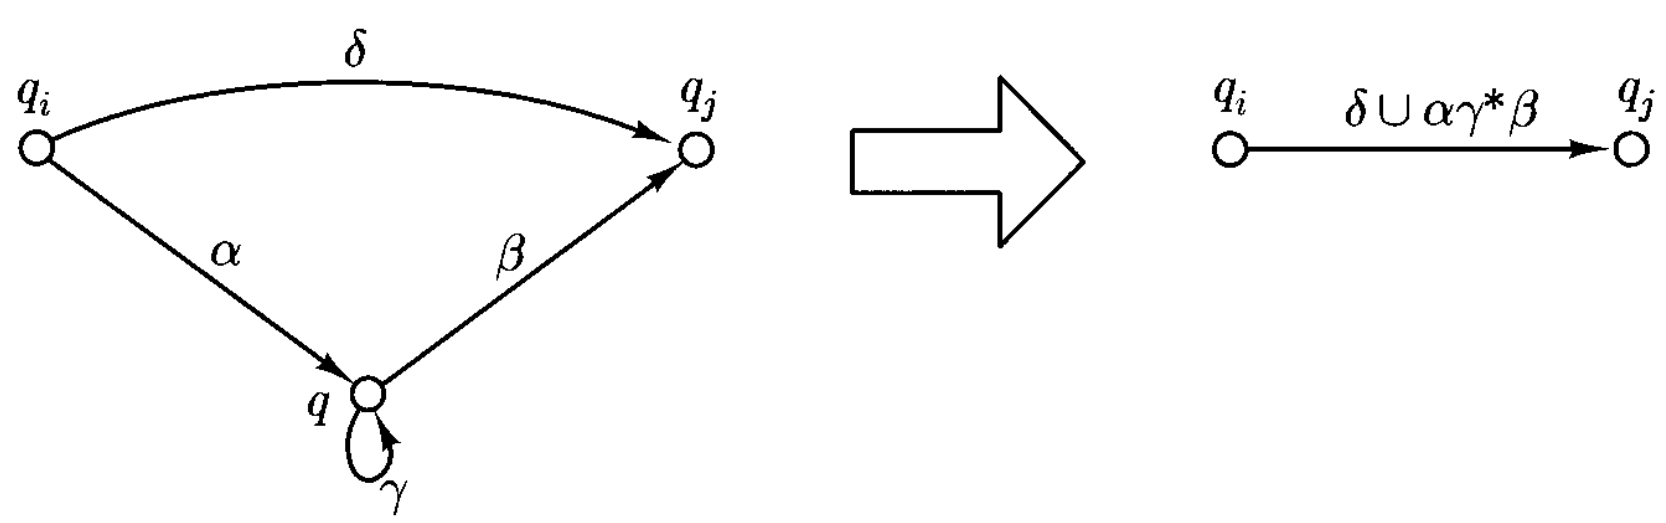
\includegraphics[width=.42\textwidth]{img/Fig2.17.png}
  \caption{}
\end{figure}


\section{Languages that are and are not Regular}

The regular languages are closed under a variety of operations and that regular languages may be specified either by regular expressions or by deterministic or nondeterministic finite automata. These facts, used singly or in combinations, provide a variety of techniques for showing languages to be regular.

\begin{example}{}
  Let $\Sigma = \{0, 1, ..., 9\}$ and let $L \subseteq \Sigma^*$ be the set of decimal representations for nonnegative integers (without redundant leading O's) divisible by 2 or 3. For example, $0, 3, 6, 244 \in L$, but $1, 03, 00 \notin L$. Then $L$ is regular. We break the proof into four parts.

  \quad Let $L_1$ be the set of decimal representations of nonnegative integers. Then it is easy to see that
  \begin{equation*}
    L_1 = 0 \cup \left\{ 1, 2, ..., 9 \right\} \Sigma^*
  \end{equation*}
  which is regular since it is denoted by a regular expression.

  \quad Let $L_2$ be the set of decimal representations of nonnegative integers divisible by 2. Then $L_2$ is just the set of members of $L$, ending in 0, 2, 4, 6, or 8; that is,
  \begin{equation*}
    L_2 = L_1 \cap \Sigma^* \left\{ 0, 2, 4, 6, 8 \right\}
  \end{equation*}
  which is regular by Theorem 2(e).

  \quad Let $L_3$ be the set of decimal representations of nonnegative integers divisible by 3. Recall that a number is divisible by 3 if and only if the sum of its digits is divisible by 3. We construct a finite automaton that keeps track in its finite control of the sum modulo 3 of a string of digits. $L_3$ will then be the intersection with $L_1$ of the language accepted by this finite automaton. The automaton is pictured in Figure 15.

  \quad Finally, $L = L_2 \cup L_3$ , surely a regular language.
\end{example}

\begin{figure}[h!]
  \centering
  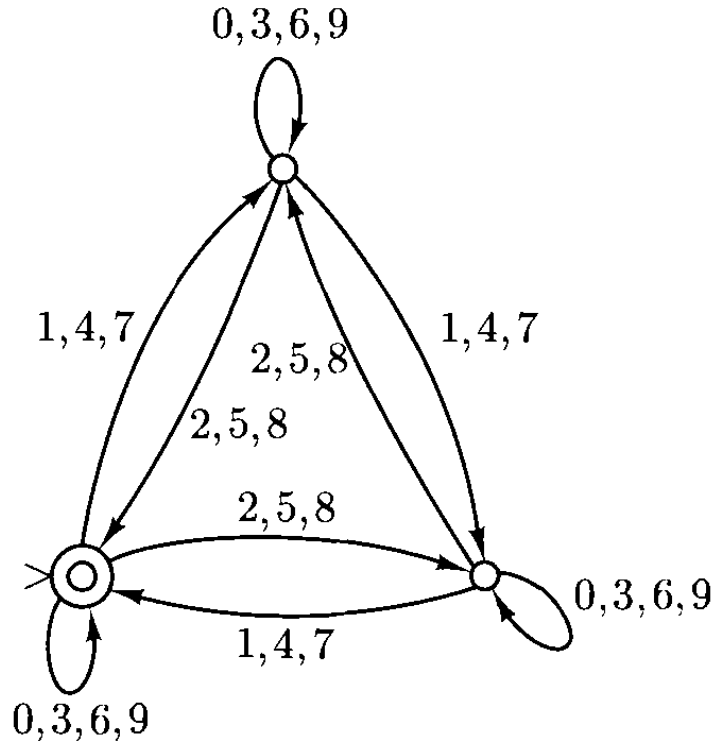
\includegraphics[width=.3\textwidth]{img/Fig2.18.png}
  \caption{}
\end{figure}

\begin{formula}{From Ebru Hoca's Notes}
  To show that a language $L$ is regular, one of the following methods can be used:
  \begin{itemize}
    \item write a regular expression $\alpha$ such that $L = L(\alpha)$
    \item construct an NFA $M$ such that $L = L(M)$
    \item use closure properties, e.g., for regular languages $L_1$ and $L_2$, show $L = L_1 \cap L_2$, $L = L_1 \cup L_2$, $L = L_1 L_2$,
    or $L = \Sigma^* \setminus L_1$ (more examples can be added)
  \end{itemize}
\end{formula}

Although we now have a variety of powerful techniques for showing that languages are regular, as yet we have none for showing that languages are not regular. Two properties shared by all regular languages, but not by certain nonregular languages, may be phrased intuitively as follows: 
\begin{enumerate}
  \item As a string is scanned left to right, the amount of memory that is required in order to determine at the end whether or not the \textit{string is in the language must be bounded}, fixed in advance and dependent on the language, not the particular input string. For example, we would expect that $\{a^n b^n\ |\ n \geq 0\}$ is not regular, since it is difficult to imagine how a finite-state device could be constructed that would correctly remember, upon reaching the border between the $a$'s and the $b$'s, how many $a$'s it had seen, so that the number could be compared against the number of $b$'s.
  \item Regular languages with an infinite number of strings are represented by automata with cycles and regular expressions involving the Kleene star. Such languages must have infinite subsets with a certain simple repetitive structure that arises from the Kleene star in a corresponding regular expression or a cycle in the state diagram of a finite automaton. This would lead us to expect, for example, that $\{a^n\ |\ n \geq 1 \textnormal{ is a prime}\}$ is not regular, since there is no simple periodicity in the set of prime numbers.
\end{enumerate}

In brief,
\begin{formula}{From Ebru Hoca's Notes}
  To show that a language $L$ is not regular, we use the following property of regular languages: 
  \begin{itemize}
    \item as a string is scanned from left to right, the amount of memory required to determine if $w \in L$ or $w \notin L$ must be bounded.
    \item In RL, infinite languages can be represented with Kleene star (cycle in automata), which induce a periodicity/pattern.
  \end{itemize}
\end{formula}

These intuitive ideas are formalized in the following theorem known as \textit{Pumping Lemma}.

\begin{theorem}{: Pumping Lemma}
  \textit{Let $L$ be a regular language. There is an integer $n \geq 1$ such that any string $w \in L$ with $|w| \geq n$ can be rewritten as $w = xyz$ such that $y \neq e$, $|xy| \leq n$ and $xy^iz \in L$ for each $i \geq 0$.}  
\end{theorem}

\begin{proof}
  Since $L$ is regular, $L$ is accepted by a deterministic finite automaton $M$. Suppose that $n$ is the number of states of $M$, and let $w$ be a string of length $n$ or greater. Consider now the first $n$ steps of the computation of $M$ on $w$:
  \begin{equation*}
    \left( q_0, w_1w_2...w_n \right) \vdash_M \left( q_1, w_2...w_n \right) \vdash_M ... \vdash_M (q_n, e)
  \end{equation*}
  where $q_0$ is the initial state of $M$, and $w_1...w_n$ are the $n$ first symbols of $w$. Since $M$ has only $n$ states, and there are $n + 1$ configurations $(q_i, w_{i+1}..., w_n)$ appearing in the computation above, by the \textit{pigeonhole principle} there exist $i$ and $j$, $0 \leq i < j \leq n$, such that $q_i = q_j$. That is, the string $y = w_iw_{i+1}...w_j$ drives $M$ from state $q_i$ back to state $q_i$, and this string is nonempty since $i < j$. But then this string could be removed from $w$, or repeated any number of times in $w$ just after the $j$th symbol of $w$, and $M$ would still accept this string. That is, $M$ accepts $xy^iz \in L$ for each $i \geq 0$, where $x = w_1...w_i$, and $z = w_{j+1}...w_m$. Notice finally that the length of $xy$, the number we called $j$ above, is by definition at most $n$, as required.

  Also, watch the following video: \href{https://youtu.be/qtnNyUlO6vU}{What is the Pumping Lemma}

  \begin{formula}{}
    \quad Assume $L$ is a regular language and there is a string $w \in L$. Now, imagine, not find or determine, that there is a integer $n$ that is $n \geq 1$, $n > 0$. Also, this integer is smaller than the length of the string $w$, $n \leq |w|$. So,
  \begin{align*}
    |w| \geq n \geq 1 && \textnormal{or} && |w| \geq n > 0
  \end{align*}
  Also, notice that the string can be written as three parts: $w = xyz$.

  If the followings are satisfied, it shows that $w \in L$ and $L$ is regular:
  \begin{itemize}
    \item $|y| > 0$: $y$ is not empty string
    \item $|xy| \leq n$: the length of the part of the string $xy$ is less than $n$
    \item $xy^iz \in L,\textnormal{ for each } i \geq 0$: When part $y$ is repeated, or pumped, as many times we want, the expression is still in language
  \end{itemize}
  In here, $x$ or $z$ can be empty string, $e$, but $y$ cannot be the empty string, $e$. Notice that the chosen part of string that will be compared with $n$ should be located in first $n$.
  \end{formula}
\end{proof}

Pumping lemma is also used to show that a language is not regular: start applying the pumping lemma, then find a contradiction.
\begin{formula}{}
\noindent For each regular language $L$,

\quad there exists $n \geq 1$ such that (this is a general term do not pick a number!!!)

\quad \quad for each $w \in L$ with $|w| \geq n$ (write a string with respect to $n$, that can be used to reach a contradiction)

\quad \quad \quad there exists $x, y, z$ with $w = xyz$, $y \neq e$, $|xy| \leq n$ (consider each possible split satisfying these constraints)

\quad \quad \quad \quad for each $i \geq 0$, $xy^iz \in L$ (show that there exists an $i$ such that $xy^iz \neq L$, contradiction)
\end{formula}

Applying the theorem correctly can be subtle. It is often useful to think of the application of this result as a \textit{game} between yourself, the prover, who is striving to establish that the given language $L$ is not regular, and an adversary who is insisting that $L$ is regular. 

\begin{formula}{}
\noindent The theorem states that, once $L$ has been fixed,

\quad the adversary must start by providing a number $n$;

\quad \quad then you come up with a string $w$ in the language that is longer than $n$, $|w| \geq n$;

\quad \quad \quad the adversary must now supply an appropriate decomposition of $w$ into $xyz$;

\quad \quad \quad \quad and, finally, you triumphantly point
out $i$ for which $xy^iz$ is not in the language.
\end{formula}

If you have a strategy that always wins, no matter how brilliantly the adversary plays, then you have established that $L$ is not regular.

\begin{example}{}
  The language $L = \{a^ib^i\ |\ i \geq 0\}$ is not regular, for if it were regular, Theorem 4 would apply for some integer $n$. Consider then the string $w = a^nb^n \in L$. By the theorem, it can be rewritten as $w = xyz$ such that $|xy| \leq n$ and $y \neq e$ -that is, $y = a^i$ for some $i > 0$. But then $xz = a^{n-i}b^n \notin L$, $y^0 = e$, contradicting the theorem.
\end{example}

\begin{example}{}
  The language $L = \{a^n\ |\ n \textnormal{ is prime}\}$ is not regular. For suppose it were, and let $x$, $y$, and $z$ be as specified in Theorem 4. Then $x = a^p$ , $y = a^q$, and $z = a^r$, where $p, r \geq 0$ and $q > 0$. By the theorem, $xy^iz \in L$ for each $i \geq 0$; that is, $p + iq + r$ is prime for each $i \geq 0$. But this is impossible; for let $i = p + 2q + r + 2$; then $p + iq + r = (q + 1) \cdot (p + 2q + r)$, which is a product of two natural numbers, each greater than 1.
\end{example}

\begin{example}{}
  Sometimes it pays to use closure properties to show that a language is not regular. Take for example
  \begin{equation*}
    L = \left\{ w \in \left\{ a, b \right\}^*\ |\ w \textnormal{ has an equal number of $a$'s and $b$'s} \right\}
  \end{equation*}
  $L$ is not regular, because if $L$ were indeed regular, then so would be $L \cap a^*b^*$ -by closure under intersection. However, this latter language is precisely ${a^nb^n\ |\ n \geq 0}$, which we just showed is not regular.
\end{example}


\section{State Minimization}

The process of reducing a given DFA to its minimal form is called as minimization of DFA.
\begin{itemize}
  \item It contains the minimum number of states.
  \item The DFA in its minimal form is called as a Minimal DFA.
\end{itemize}

The two popular methods for minimizing a DFA are
\begin{itemize}
  \item Equivalence Theorem
  \item Myhill Nerode Theorem
\end{itemize}

\newpage
\subsection{Equivalence Theorem}

\begin{multicols}{2}
\setlength{\columnsep}{1.5cm}
\setlength{\columnseprule}{0.2pt}

\subsubsection*{Step-1}

Eliminate all the dead states and inaccessible states from the given DFA (if any).

\begin{itemize}
  \item \textbf{Dead State:} All those non-final states which transit to itself for all input symbols in $\Sigma$ are called as dead states.
  \item \textbf{Inaccessible State:} All those states which can never be reached from the initial state are called as inaccessible states.
\end{itemize}

\subsubsection*{Step-2}

Draw a state transition table for the given DFA. Transition table shows the transition of all states on all input symbols in $\Sigma$.

\subsubsection*{Step-3}

Now, start applying equivalence theorem.
\begin{itemize}
  \item Take a counter variable $k$ and initialize it with value 0.
  \item Divide $Q$ (\textit{set of states}) into two sets such that one set contains all the non-final states and other set contains all the final states.
  \item This partition is called $P_0$.
\end{itemize}

\subsubsection*{Step-4}

\begin{itemize}
  \item Increment $k$ by $1$.
  \item Find $P_k$ by partitioning the different sets of $P_{k - 1}$.
  \item In each set of $P_{k - 1}$, consider all the possible pair of states within each set and if the two states are distinguishable, partition the set into different sets in $P_k$.
\end{itemize}

Two states $q_1$ and $q_2$ are distinguishable in partition $P_k$ for any input symbol `$a$', if $\delta(q_1, a)$ and $\delta(q_2, a)$ are in different sets in partition $P_{k-1}$.

\subsubsection*{Step-5}

Repeat \textit{step-4} until no change in partition occurs. In other words, when you find $P_k = P_{k - 1}$, stop.

\subsubsection*{Step-6}

All those states which belong to the same set are equivalent. The equivalent states are merged to form a single state in the minimal DFA.

\begin{center}
  \textit{\# of states in Minimal DFA = \# of sets in $P_k$  }
\end{center}

\end{multicols}

\begin{examplebreak}{}
  Minimize the following DFA:
  \begin{center}
    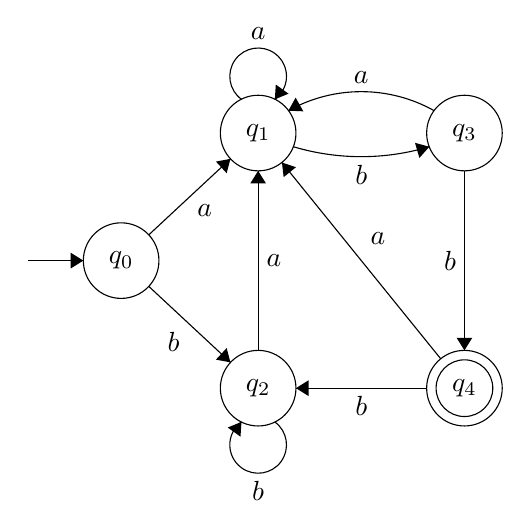
\begin{tikzpicture}[scale=0.2]
    \tikzstyle{every node}+=[inner sep=0pt]
    \draw [black] (6.1,-15.4) circle (2.4);
    \draw (6.1,-15.4) node {$q_0$};
    \draw [black] (14.8,-7.3) circle (2.4);
    \draw (14.8,-7.3) node {$q_1$};
    \draw [black] (14.8,-23.5) circle (2.4);
    \draw (14.8,-23.5) node {$q_2$};
    \draw [black] (27.9,-7.3) circle (2.4);
    \draw (27.9,-7.3) node {$q_3$};
    \draw [black] (27.9,-23.5) circle (2.4);
    \draw (27.9,-23.5) node {$q_4$};
    \draw [black] (27.9,-23.5) circle (1.8);
    \draw [black] (7.86,-13.76) -- (13.04,-8.94);
    \fill [black] (13.04,-8.94) -- (12.12,-9.11) -- (12.8,-9.85);
    \draw (11.41,-11.83) node [below] {$a$};
    \draw [black] (7.86,-17.04) -- (13.04,-21.86);
    \fill [black] (13.04,-21.86) -- (12.8,-20.95) -- (12.12,-21.69);
    \draw (9.43,-19.93) node [below] {$b$};
    \draw [black] (25.665,-8.168) arc (-73.33794:-106.66206:15.05);
    \fill [black] (25.67,-8.17) -- (24.76,-7.92) -- (25.04,-8.88);
    \draw (21.35,-9.3) node [below] {$b$};
    \draw [black] (27.9,-9.7) -- (27.9,-21.1);
    \fill [black] (27.9,-21.1) -- (28.4,-20.3) -- (27.4,-20.3);
    \draw (27.4,-15.4) node [left] {$b$};
    \draw [black] (0.2,-15.4) -- (3.7,-15.4);
    \fill [black] (3.7,-15.4) -- (2.9,-14.9) -- (2.9,-15.9);
    \draw [black] (13.742,-5.156) arc (234:-54:1.8);
    \draw (14.8,-1.4) node [above] {$a$};
    \fill [black] (15.86,-5.16) -- (16.73,-4.8) -- (15.92,-4.22);
    \draw [black] (16.724,-5.877) arc (119.23219:60.76781:9.472);
    \fill [black] (16.72,-5.88) -- (17.67,-5.92) -- (17.18,-5.05);
    \draw (21.35,-4.17) node [above] {$a$};
    \draw [black] (26.39,-21.63) -- (16.31,-9.17);
    \fill [black] (16.31,-9.17) -- (16.42,-10.1) -- (17.2,-9.47);
    \draw (21.91,-13.97) node [right] {$a$};
    \draw [black] (14.8,-21.1) -- (14.8,-9.7);
    \fill [black] (14.8,-9.7) -- (14.3,-10.5) -- (15.3,-10.5);
    \draw (15.3,-15.4) node [right] {$a$};
    \draw [black] (25.5,-23.5) -- (17.2,-23.5);
    \fill [black] (17.2,-23.5) -- (18,-24) -- (18,-23);
    \draw (21.35,-24) node [below] {$b$};
    \draw [black] (15.858,-25.644) arc (54:-234:1.8);
    \draw (14.8,-29.4) node [below] {$b$};
    \fill [black] (13.74,-25.64) -- (12.87,-26) -- (13.68,-26.58);
    \end{tikzpicture}
  \end{center}

  \textbf{Solution:}

  \begin{itemize}
    \item Step - 1:
      The given DFA contains no dead states and inaccessible states.

    \item Step - 2:
      Draw a state transition table
        \begin{center}
          \begin{tabular}{c|c|c}
          $\delta$  & $a$    & $b$     \\ 
          \hline
          $q_0$  & $q_1$  & $q_2$  \\
          $q_1$  & $q_1$  & $q_3$  \\
          $q_2$  & $q_1$  & $q_2$  \\
          $q_3$  & $q_1$  & $q_4$  \\
          $q_4$  & $q_1$  & $q_2$ 
          \end{tabular}
        \end{center}
    
    \item Step - 3:
      Now using Equivalence Theorem, we have:
      \begin{itemize}
        \item $P_0 = \{ q_0 , q_1 , q_2 , q_3 \}, \{ q_4 \}$
        \item $P_1 = \{ q_0 , q_1 , q_2 \}, \{ q_3 \}, \{ q_4 \}$
        \item $P_2 = \{ q_0 , q_2 \}, \{ q_1 \}, \{ q_3 \}, \{ q_4 \}$
        \item $P_3 = \{ q_0 , q_2 \}, \{ q_1 \}, \{ q_3 \}, \{ q_4 \}$
      \end{itemize}

      Since $P_3 = P_2$, so we stop. From $P_3$, we infer that states $q_0$ and $q_2$ are equivalent and can be merged together.
    
    \item So, Our minimal DFA is
      \begin{multicols}{2}
        \begin{center}
          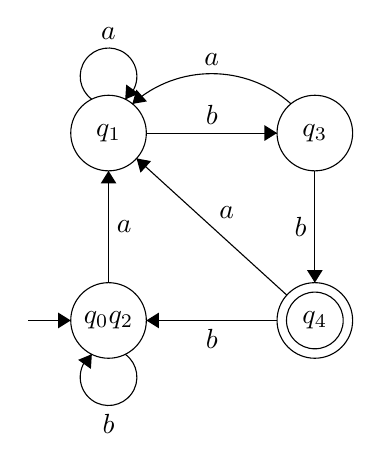
\begin{tikzpicture}[scale=0.2]
            \tikzstyle{every node}+=[inner sep=0pt]
            \draw [black] (5.3,-19.2) circle (2.4);
            \draw (5.3,-19.2) node {$q_0q_2$};
            \draw [black] (5.3,-7.3) circle (2.4);
            \draw (5.3,-7.3) node {$q_1$};
            \draw [black] (18.4,-7.3) circle (2.4);
            \draw (18.4,-7.3) node {$q_3$};
            \draw [black] (18.4,-19.2) circle (2.4);
            \draw (18.4,-19.2) node {$q_4$};
            \draw [black] (18.4,-19.2) circle (1.8);
            \draw [black] (5.3,-16.8) -- (5.3,-9.7);
            \fill [black] (5.3,-9.7) -- (4.8,-10.5) -- (5.8,-10.5);
            \draw (5.8,-13.25) node [right] {$a$};
            \draw [black] (7.7,-7.3) -- (16,-7.3);
            \fill [black] (16,-7.3) -- (15.2,-6.8) -- (15.2,-7.8);
            \draw (11.85,-6.8) node [above] {$b$};
            \draw [black] (18.4,-9.7) -- (18.4,-16.8);
            \fill [black] (18.4,-16.8) -- (18.9,-16) -- (17.9,-16);
            \draw (17.9,-13.25) node [left] {$b$};
            \draw [black] (0.2,-19.2) -- (2.9,-19.2);
            \fill [black] (2.9,-19.2) -- (2.1,-18.7) -- (2.1,-19.7);
            \draw [black] (4.242,-5.156) arc (234:-54:1.8);
            \draw (5.3,-1.4) node [above] {$a$};
            \fill [black] (6.36,-5.16) -- (7.23,-4.8) -- (6.42,-4.22);
            \draw [black] (6.81,-5.448) arc (131.72779:48.27221:7.572);
            \fill [black] (6.81,-5.45) -- (7.74,-5.29) -- (7.07,-4.54);
            \draw (11.85,-3.03) node [above] {$a$};
            \draw [black] (16.62,-17.59) -- (7.08,-8.91);
            \fill [black] (7.08,-8.91) -- (7.33,-9.82) -- (8,-9.08);
            \draw (12.81,-12.76) node [above] {$a$};
            \draw [black] (6.358,-21.344) arc (54:-234:1.8);
            \draw (5.3,-25.1) node [below] {$b$};
            \fill [black] (4.24,-21.34) -- (3.37,-21.7) -- (4.18,-22.28);
            \draw [black] (16,-19.2) -- (7.7,-19.2);
            \fill [black] (7.7,-19.2) -- (8.5,-19.7) -- (8.5,-18.7);
            \draw (11.85,-19.7) node [below] {$b$};
          \end{tikzpicture}
        \end{center}

        \vfill\null
        \columnbreak

        \begin{center}
          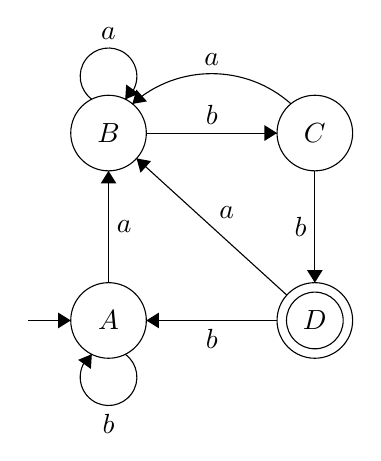
\begin{tikzpicture}[scale=0.2]
            \tikzstyle{every node}+=[inner sep=0pt]
            \draw [black] (5.3,-19.2) circle (2.4);
            \draw (5.3,-19.2) node {$A$};
            \draw [black] (5.3,-7.3) circle (2.4);
            \draw (5.3,-7.3) node {$B$};
            \draw [black] (18.4,-7.3) circle (2.4);
            \draw (18.4,-7.3) node {$C$};
            \draw [black] (18.4,-19.2) circle (2.4);
            \draw (18.4,-19.2) node {$D$};
            \draw [black] (18.4,-19.2) circle (1.8);
            \draw [black] (5.3,-16.8) -- (5.3,-9.7);
            \fill [black] (5.3,-9.7) -- (4.8,-10.5) -- (5.8,-10.5);
            \draw (5.8,-13.25) node [right] {$a$};
            \draw [black] (7.7,-7.3) -- (16,-7.3);
            \fill [black] (16,-7.3) -- (15.2,-6.8) -- (15.2,-7.8);
            \draw (11.85,-6.8) node [above] {$b$};
            \draw [black] (18.4,-9.7) -- (18.4,-16.8);
            \fill [black] (18.4,-16.8) -- (18.9,-16) -- (17.9,-16);
            \draw (17.9,-13.25) node [left] {$b$};
            \draw [black] (0.2,-19.2) -- (2.9,-19.2);
            \fill [black] (2.9,-19.2) -- (2.1,-18.7) -- (2.1,-19.7);
            \draw [black] (4.242,-5.156) arc (234:-54:1.8);
            \draw (5.3,-1.4) node [above] {$a$};
            \fill [black] (6.36,-5.16) -- (7.23,-4.8) -- (6.42,-4.22);
            \draw [black] (6.81,-5.448) arc (131.72779:48.27221:7.572);
            \fill [black] (6.81,-5.45) -- (7.74,-5.29) -- (7.07,-4.54);
            \draw (11.85,-3.03) node [above] {$a$};
            \draw [black] (16.62,-17.59) -- (7.08,-8.91);
            \fill [black] (7.08,-8.91) -- (7.33,-9.82) -- (8,-9.08);
            \draw (12.81,-12.76) node [above] {$a$};
            \draw [black] (6.358,-21.344) arc (54:-234:1.8);
            \draw (5.3,-25.1) node [below] {$b$};
            \fill [black] (4.24,-21.34) -- (3.37,-21.7) -- (4.18,-22.28);
            \draw [black] (16,-19.2) -- (7.7,-19.2);
            \fill [black] (7.7,-19.2) -- (8.5,-19.7) -- (8.5,-18.7);
            \draw (11.85,-19.7) node [below] {$b$};
          \end{tikzpicture}
        \end{center}
      \end{multicols}
  \end{itemize}
\end{examplebreak}


\subsection{Myhill Nerode Theorem}

\begin{multicols}{2}
\setlength{\columnsep}{1.5cm}
\setlength{\columnseprule}{0.2pt}

\begin{enumerate}
  \item Create the pairs of all the states involved in the given DFA.
  \item Mark all the pairs $(Q_a, Q_b)$ such a that $Q_a$ is Final state and $Q_b$ is Non-Final State or vice versa.
  \item If there is any unmarked pair $(Q_a, Q_b)$ such a that $\delta(Q_a, x)$ and $\delta(Q_b, x)$ is marked, then mark $(Q_a, Q_b)$. Here $x$ is a input symbol. Repeat this step until no more marking can be made.
  \item Combine all the unmarked pairs and make them a single state in the minimized DFA.
\end{enumerate}

\vfill\null
\columnbreak

This way is quite cumbersome and prone to errors. Check the following links for examples:

\begin{figure}[H]
  \centering
  
\includegraphics[width=.2\textwidth]{img/minizimation-1.png}
  \caption{\href{https://bit.ly/3xVGyMD}{https://bit.ly/3xVGyMD}}
\end{figure}

\begin{figure}[H]
  \centering
  
\includegraphics[width=.2\textwidth]{img/minizimation-2.png}
  \caption{\href{https://bit.ly/3Oxj9Xw}{https://bit.ly/3Oxj9Xw}}
\end{figure}

\end{multicols}


% \section{State Minimization (Book)}

It is important to be able to \textit{minimize the number of states} of a given deterministic finite automaton, that is, to determine an equivalent deterministic finite automaton that has as few states as possible. We shall next develop the necessary concepts and results that lead to such a \textit{state minimization algorithm}.

\begin{figure}[h!]
  \centering
  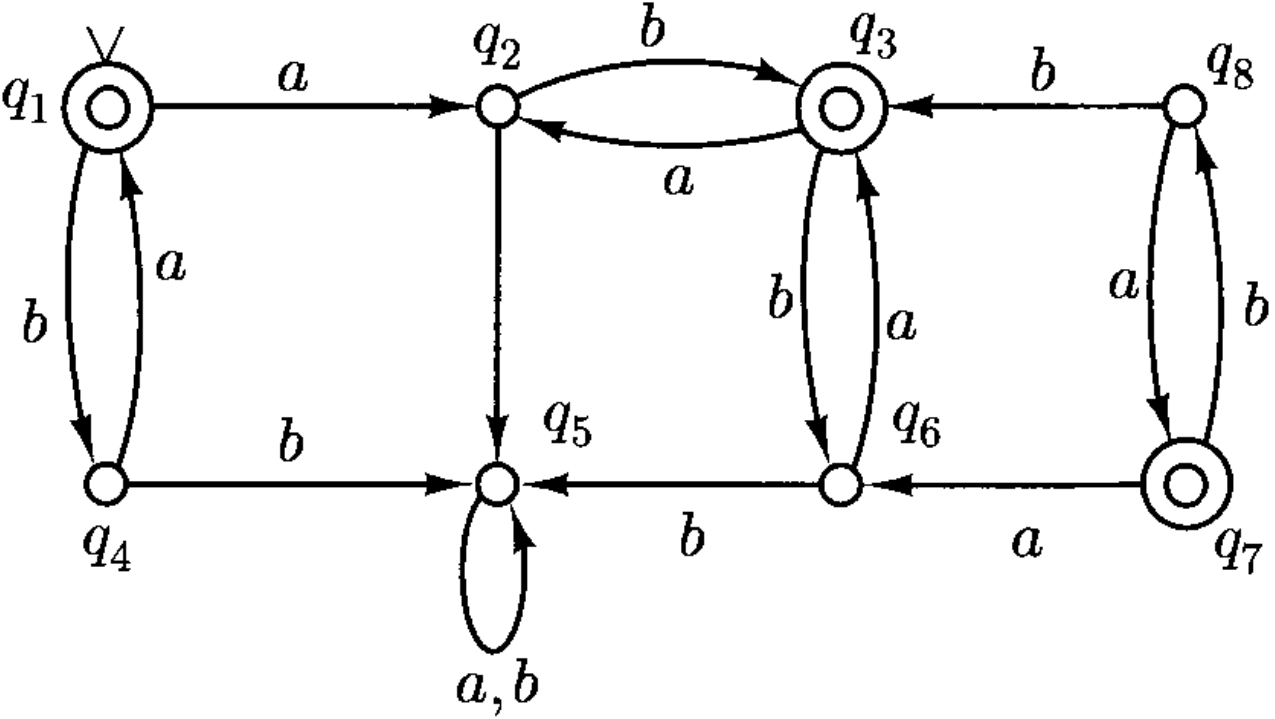
\includegraphics[width=.4\textwidth]{img/Fig2.19.png}
  \caption{}
\end{figure}

Given a deterministic finite automaton, there may be an easy way to get rid of several states. Let us take, for example, the deterministic automaton in Figure 16, accepting the language $L = (ab \cup ba)^*$. 

Consider state $q_7$. It should be clear that this state is \textit{unreachable}, because there is no path from the start state to it in the state diagram of the automaton. This is the simplest kind of optimization one can do on any deterministic finite automaton:\textit{ Remove all unreachable states and all transitions in and out of them}. In fact, this optimization was implicit in our conversion of a nondeterministic finite automaton to its equivalent deterministic one: We omitted from consideration all states that are not reachable from the start state of the resulting automaton.

Identifying the reachable states is easy to do in polynomial time, because the set of reachable states can be defined as the closure of $\{s\}$ under the relation $\left\{ (p, q)\ |\ \delta(p, a) = q \textnormal{ for some } a \in \Sigma \right\}$. Therefore,the set of all reachable states can be computed by this simple algorithm.

\begin{algorithm}
  \begin{algorithmic}
    \State $R$ := $\{s\}$
    \While{there is a state $p \in R$ and $a \in \Sigma$ such that $\delta(p, a) \notin R$}
      \State add $\delta(p, a)$ to $R$
    \EndWhile
\end{algorithmic}
\end{algorithm}

\begin{figure}[h!]
  \centering
  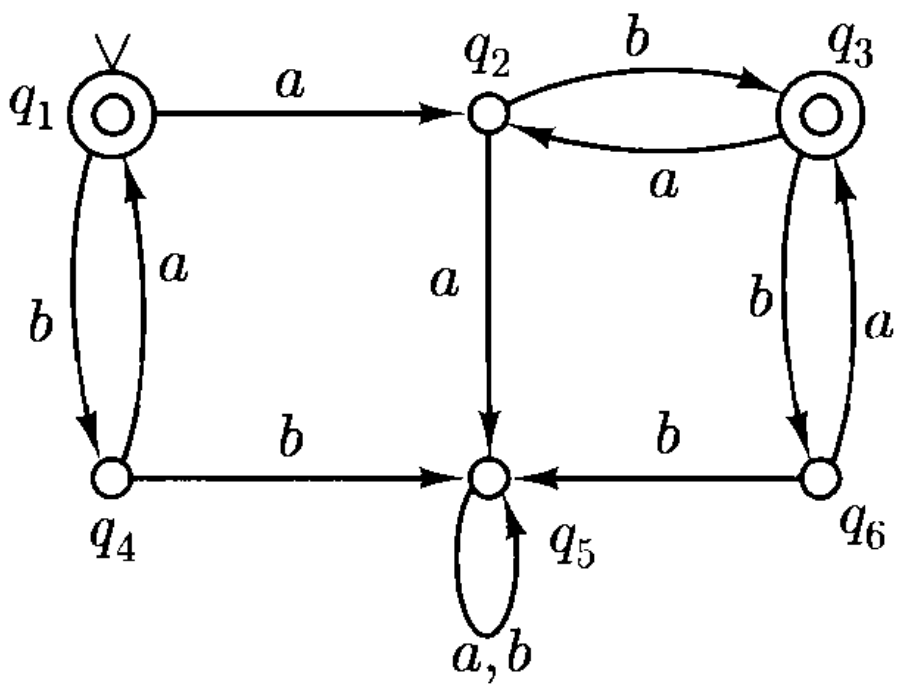
\includegraphics[width=.3\textwidth]{img/Fig2.20.png}
  \caption{}
\end{figure}

However, the remaining automaton after the deletion of unreachable states (Figure 17) still has more states than are really needed, this time for subtler reasons. For example, states $q_4$ and $q_6$ are equivalent, and therefore they \textit{can be merged into one state}. What does this mean, exactly? Intuitively, the reason we call these states equivalent is that, from \textit{either state, precisely the same strings lead the automaton to acceptance}.

\begin{definition}{}
  Let $L \subseteq \Sigma^*$ be a language, and let $x, y \in \Sigma^*$. We say that $x$ and $y$ are \textbf{equivalent with respect to $L$}, denoted $x \approx_L y$, if for all $z \in \Sigma^*$, the following is true: $xz \in L$ if and only if $yz \in L$. Notice that $\approx_L$ is an equivalence relation. 
\end{definition}

That is, $x \approx_L y$ if either both strings belong to $L$ or neither is in $L$; and moreover, appending any fixed string to both $x$ and $y$ results in two strings that are either both in $L$ or both not in $L$. (In other words, if $x \approx_L y$, then either $x, y \in L$ or $x, y \notin L$ (why?). In addition, if $x \approx_L y$, then appending the same string $z$ to both of them results in two strings that are either both in $L$ or both not in $L$.)

\begin{example}{}
  If $x$ is a string, and when $L$ is understood by context, we denote by $\left[ x \right]$ the equivalence class with respect to $L$ to which $x$ belongs. For example, for the language $L = (ab \cup ba)^*$ accepted by the automaton in Figure 17, it is not hard to see that $\approx_L$ has four equivalence classes:
  \begin{itemize}
    \item $\left[ e \right] = L$
    \item $\left[ a \right] = La$
    \item $\left[ b \right] = Lb$
    \item $\left[ aa \right] = L(aa \cup bb) \Sigma^*$
  \end{itemize}
  In (1), for any string $x \in L$, including $x = e$, the $z$'s that make $xz \in L$ are precisely the members of $L$. In (2), any $x \in La$ needs a $z$ of the form $bL$ in order for $xz$ to be in $L$. Similarly, for (3) the $z$'s are of the form $aL$. Finally, in (4) there is no $z$ that can restore to $L$ a string with a prefix in $L(aa \cup bb)$. In other words, all strings in set (1) have the same fate with respect to inclusion in $L$; and the same for (2), (3), and (4). Finally, it is easy to see that these four classes exhaust all of $\Sigma^*$. Hence these are the equivalence classes of $\approx_L$.
\end{example}

Notice that $\approx_L$ relates strings in terms of a language, not in terms of an automaton. Automata provide another, somewhat less fundamental, relation, described next.

\begin{definition}{}
  Let $M = (K, \Sigma, \delta, s, F)$ be a deterministic finite automaton. We say that two strings $x, y \in \Sigma^*$ are \textbf{equivalent with respect} to $M$, denoted $x \sim_M y$, if, intuitively, they both drive $M$ from $s$ to the same state. Formally, $x \sim_M y$ if there is a state $q$ such that $(s, x) \vdash_M^* (q, e)$ and $(s, y) \vdash_M^* (q, e)$.

  \quad Again, $\sim_M$ is an equivalence relation. Its equivalence classes can be identified by the states of $M$ -more precisely, with \textbf{\textit{those states that are reachable from $s$ and therefore have at least one string in the corresponding equivalence class}}. We denote the equivalence class corresponding to state $q$ of $M$ as $E_q$.
\end{definition}

\setcounter{example}{9}
\begin{example}{ continued}
  For example, for the automaton $M$ in Figure 17, the equivalence classes of $\sim_M$ are these (where $L = (ab \cup ba)^*$ is the language accepted by $M$)
  \begin{enumerate}
    \item $E_{q_1} = (ba)^*$ (by reading, $q_1$ is reachable from $s$)
    \item $E_{q_2} = La \cup a$ (by reading, $q_2$ is reachable from $s$)
    \item $E_{q_3} = abL$ (by reading, $q_3$ is reachable from $s$ and so on)
    \item $E_{q_4} = b (ab)^*$
    \item $E_{q_5} = L(bb \cup aa)\Sigma^*$
    \item $E_{q_6} = abLb$
  \end{enumerate}
  Again, they form a partition of $\Sigma^*$.
\end{example}

These two important equivalence relations, one associated with the language, the other with the automaton, are related as follows:

\begin{theorem}{}
  For any deterministic finite automaton $M = \left( K, \Sigma, \delta, s, F \right)$ and any strings $x, y \in \Sigma^*$, if $x \sim_M y$, then $x \approx_{L(M)} y$.   
\end{theorem}

\begin{proof}
  For any string $x \in \Sigma^*$, let $q(x) \in K$ be the unique state such that $(s, x) \vdash_M^* (q(x), e)$. Notice that, for any $x,z \in \Sigma^*$, $xz \in L(M)$ if and only if $(q(x), z) \vdash_M^* (f,e)$ for some $f \in F$. Now, if $x \sim_M y$ then, by the definition of $\sim_M$, $q(x) = q(y)$, and thus $x \sim_M y$ implies that the following holds:
  \begin{equation*}
    xz \in L(M) \textnormal{ if and only if } yz \in L(M) \textnormal{ for all } z \in \Sigma^*
  \end{equation*}
  which is the same as $x \approx_{L(M)} y$.
\end{proof}

A very suggestive way of expressing Theorem 5 is to say that $\sim_M$ is
a \textbf{refinement} of $\approx_{L(M)}$. In general, we say that an equivalence relation $\sim$ is a refinement of another $\approx$ if for all $x, y$ $x \sim y$ implies $x \approx y$. If $\sim$ is a refinement of $\approx$, then each equivalence class with respect to $\approx$ is contained in some equivalence class of $\approx$; that is, each equivalence class of $\approx$ is the union of one or more equivalence classes of $\sim$.

\setcounter{example}{9}
\begin{example}{ continued}
  For an example that is more to the point, the equivalence classes of $\sim_M$ for the automaton $M$ in Figure 17 ``refine'' in this sense the equivalence classes of $\approx_{L(M)}$, exactly as predicted by Theorem 5. For example, classes $E_{q_5}$ and $\left[aa\right]$ coincide, while classes $E_{q_1}$ and $E_{q_3}$ are both subsets of $\left[ e \right]$.
\end{example}

Theorem 5 implies something very important about $M$ and any other automaton $M'$ accepting the same language $L(M)$: Its number of states must be at least as large as the number of equivalence classes of $L(M)$ under $\approx_{L(M)}$. Thus, the number of equivalence classes of $\approx_{L(M)}$ gives a lower bound on the number of states of an automaton $M'$ that accepts $L(M)$.

\begin{theorem}{: The Myhill-Nerode Theorem}
  Let $L \subseteq \Sigma^*$ be a regular language. Then there is a deterministic finite automaton $M = (K, \Sigma, \delta, s, F)$ with precisely as many states as there are equivalence classes in $\approx_L$ that accepts $L$. In other words, $L = L(M)$and $|K|$ is the number of equivalence classes of $\approx_L$.
\end{theorem}

\begin{multicols}{2}
\setlength{\columnsep}{1.5cm}
\setlength{\columnseprule}{0.2pt}
\begin{proof}
  As before, we denote the equivalence class of string $x \in \Sigma^*$ in the equivalence relation $\approx_L$ by $\left[x\right]$. Given $L$, we shall construct a deterministic finite automaton (the \textbf{standard automaton} for $L$) $M = (K, \Sigma, \delta, s, F)$ such that $L = L(M)$. $M$ is defined as follows:
  \begin{itemize}
    \item $K = \left\{ \left[x\right] : x \in \Sigma^*\right\}$, the set of equivalence classes under $\approx_L$.
    \item $s = \left[e\right]$, the equivalence class of $e$ under $\approx_L$.
    \item $F = \left\{ \left[ x \right] : x \in L \right\}$
    \item Finally, for any $\left[ x \right] \in K$ and any $a \in \Sigma$, define $\delta(\left[ x \right], a) = \left[ xa \right]$.
  \end{itemize}
  How do we know that the set $K$ is finite, that is, that $\approx_L$ has finitely many equivalent classes? $L$ is regular, and so it is surely accepted by some deterministic finite automaton $M'$. By the previous theorem, $\sim_{M'}$ is a refinement of $\approx_L$, and so there are fewer equivalence classes in $L$ than there are equivalence classes of $\sim_{M'}$ -that is to say, states of $M'$. Hence $K$ is a finite set. We also have to argue that $\delta$ is \textit{well defined}, that is, $\delta(\left[ x \right], a) = \left[ xa \right]$ is independent of the string $x \in \left[ x \right]$. But this is easy to see, because $x \approx_L x'$ if and only if $xa \approx_L x'a$.

  We next show that $L = L(M)$. First we show that for all $x, y \in \Sigma^*$, we have
  \begin{equation}
    \left( \left[ x \right], y \right) \vdash_M^* \left( \left[ xy \right], e \right)
  \end{equation}
  This is established by induction on $|y|$. It is trivial when $y = e$, and, if it holds for all $y$'s of length up to $n$ and $y = y'a$, then by induction $\left( \left[ x \right], y'a \right) \vdash_M^* \left( \left[ xy' \right], a \right) \vdash_M^* \left( \left[ xy \right], e \right)$.
  
  Now (1) completes the proof: For all $x \in \Sigma^*$, we have that $x \in L(M)$ if and only if $\left( \left[ e \right], x \right) \vdash *\left( q, e \right)$ for some $q \in F$, which is by (1) the same as saying $\left[ x \right] \in F$, or, by the deinition of $F$, $\left[ x \in L \right]$.
\end{proof}
\end{multicols}

\setcounter{example}{9}
\begin{example}{ continued}
  The standard automaton corresponding to the language $L = (ab \cup ba)^*$ accepted by the six-state deterministic finite automaton in Figure 17 is shown in Figure 18. It has \textit{four} states. Naturally, it is the smallest deterministic finite automaton that accepts this language.
\end{example}

\begin{figure}[h]
  \centering
  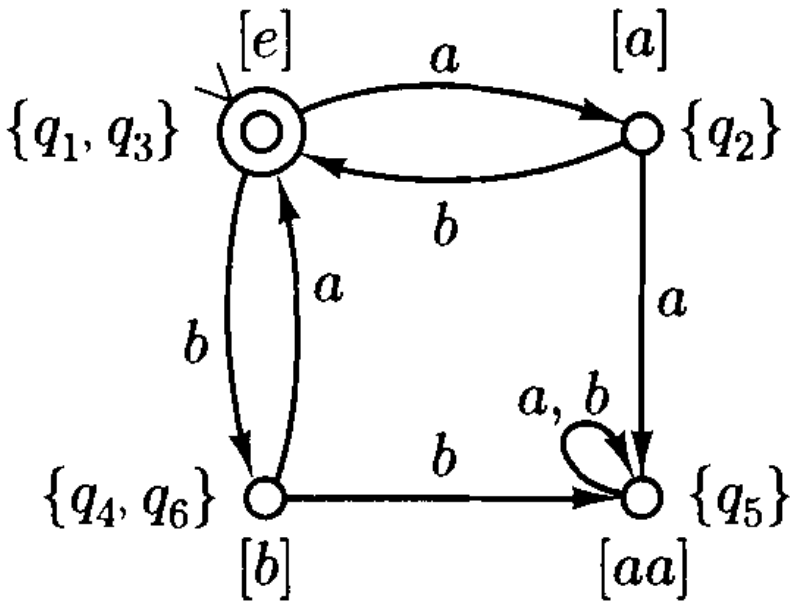
\includegraphics[width=.5\textwidth]{img/Fig2.21.png}
  \caption{}
\end{figure}

Incidentally, Theorems 6 immediately imply the following characterization of regular languages, sometimes itself called the \textit{Myhill-Nerode Theorem}:

\begin{formula}{Corollary}
  \textit{A language $L$ is regular if and only if $\approx_L$ has finitely many equivalence classes.}
\end{formula}

\begin{proof}
  If $L$ is regular, then $L = L(M)$ for some deterministic finite automaton $M$, and $M$ has at least as many states as $\approx_L$ has equivalence classes. Hence there are finitely many equivalence classes in $\approx_L$.

  \quad Conversely, if $\approx_L$ has finitely many equivalence classes, then the standard deterministic finite automaton $M_L$ (recall the proof of Theorem 6) accepts $L$.
\end{proof}

The corollary can be used to show that a language is not regular (show that it has infinitely many equivalence classes).

\begin{example}{}
  The corollary just proved is an interesting alternative way of specifying what it means for a language $L$ to be regular. Furthermore, it provides another useful way for proving that a language is not regular -besides the Pumping Theorem.

  For example, here is an alternative proof that $L = \{a^nb^n : n \geq 1\}$ is not regular: No two strings $a^i$ and $a^j$, with $i \neq j$, are equivalent under $\approx_L$, simply because there is a string (namely, $b^i$) which, when affixed $a^i$ gives a string in $L$, but when affixed to $a^j$ produces a string not in $L$. Hence $\approx_L$ has infinitely
  many equivalence classes $\left[ e \right], \left[ a \right], \left[ aa \right], \left[ aaa \right], ...$, and hence by the corollary $L$ is
  not regular.
\end{example}

\begin{multicols}{2}
\setlength{\columnsep}{1.5cm}
\setlength{\columnseprule}{0.2pt}
  For any regular language $L$ the automaton constructed in the proof of Theorem 6 is the deterministic automaton with the \textit{fewest states} that accepts $L$. Unfortunately, this automaton is defined in terms of the equivalence classes of $\approx_L$, and it is not clear how these equivalence classes can be identified for any given regular language $L$. We shall next develop an \textit{algorithm} for constructing this minimal automaton, starting from \textit{any deterministic finite automaton $M$} such that $L = L(M)$.
  
  Let $M = (K, \Sigma, \delta, s, F)$ be a deterministic finite automaton. Define a relation $A_M \subseteq K \times \Sigma^*$, as follows: $(q, w) \in A_M$ if and only if $(q, w) \vdash_M^* (f, e)$ for some $f \in F$; that is, $(q, w) \in A_M$ means that $w$ drives $M$ from $q$ to an accepting state. 
  
  Let us call two states $q, p \in K$ \textbf{equivalent}, denoted $q \equiv p$, if the following holds for all $z \in \Sigma^*$: $(q, z) \in A_M$ if and only if $(p, z) \in A_M$. Thus, if two states are equivalent, then the corresponding equivalence classes of $\sim_M$ are subsets of the same equivalence class of $\approx_L$.
  
  In other words, the equivalence classes of $\equiv$ are precisely those sets of states of $M$ that must be clumped together in order to obtain the standard automaton of $L(M)$.
  
  We shall develop an algorithm for computing the equivalence classes of $\equiv$. Our algorithm will compute $\equiv$ as the \textit{limit} of a sequence of equivalence relations $\equiv_0, \equiv_1, \equiv_2, ...$, defined next. For two states $q, p \in K$, $q \equiv_n p$ if the following is true: $(q, z) \in A_M$ if and only if $(p, z) \in A_M$ for all strings $z$ such that $|z| \leq n$. In other words, $\equiv_n$ is a \textit{coarser} equivalence relation than $\equiv$, only requiring that states $q$ and $p$ behave the same with respect to acceptance when driven by strings of \textit{length up to $n$}.

  Obviously, each equivalence relation in $\equiv_0, \equiv_1, \equiv_2, ...$ is a refinement of the previous one. Also, $q \equiv_0 p$ holds if $q$ and $p$ are either both accepting, or both non-accepting. That is, there are precisely two equivalence classes of $\equiv_0$: $F$ and $K - F$ (assuming they are both nonempty). It remains to show how $\equiv_{n+1}$ depends on $\equiv_n$. Here is how:
\end{multicols}

\begin{formula}{Lemma 1}
  \textit{For any two states $q, p \in K$ and any integer $n \geq 1$, $q \equiv_n p$ if and only if}
  \begin{enumerate}[label=\alph*)]
    \item $q \equiv_{n-1} p$, and 
    \item for all $a \in \Sigma$, $\delta(q, a) \equiv_{n-1} \delta(p, a)$.
  \end{enumerate}

  [Basically, there should be a string $z$ such that $(q, z) \in A_M$ and $(p, z) \in A_M$. To be inside $A_M$, there should be strings $w, w'$ such that $(q, w) \vdash_M^* (f,e)$ and $(p, w') \vdash_M^* (f,e)$. So if $q \equiv_{n-1} p$, and there is transition from $q$ and $p$, they can reach the step $n$.]
\end{formula}

\begin{proof}
  By definition of $\equiv_n$, $q \equiv_n p$ if and only if $q \equiv_{n-1} p$, and furthermore any string $w = av$ of length precisely $n$ drives either both $q$ and $p$ to acceptance, or both to nonacceptance. However, the second condition is the same as saying that $\delta(q, a) \equiv_{n-1} \delta(p, a)$ for any $a \in \Sigma$.
\end{proof}

Lemma 1 suggests that we can compute $\equiv$, and from this the standard
automaton for $L$, by the following algorithm:

\begin{algorithm}
  \begin{algorithmic}
    \State \texttt{Initially the equivalence classes of $\equiv_0$ are $F$ and $K - F$}
    \While{$\equiv_n\ \neq\ \equiv_{n-1}$} 
      \Comment{Repeat for $n := 1,2, ...$ until $\equiv_n$ is the same as $\equiv_{n-1}$.}
      \State \texttt{Compute the equivalence classes of $\equiv_n$ from those $\equiv_{n-1}$}
      \State (for each $a \in \Sigma$, and equivalence class $[q]$, compute $\{ \delta(q', a)\ |\ q' \in [q] \}$, and split the equivalence classes that intersect with this set)
    \EndWhile
\end{algorithmic}
\end{algorithm}

Each iteration can be carried out by applying Lemma 1: For each pair of states of $M$, we test whether the conditions of the lemma hold, and if so we put the two states in the same equivalence class of $\equiv_n$.

But how do we know that this is an algorithm, that the iteration will eventually terminate? The answer is simple: For each iteration at which the termination condition is not satisfied, ($\equiv_n\ \neq\ \equiv_{n-1}$), $\equiv_n$ is a \textit{proper refinement} of $\equiv_{n-1}$, and thus has at least one more equivalence class than $\equiv_{n-1}$. Since the number of equivalence classes cannot become more than the number of states of $M$, the algorithm will terminate after at most $|K| - 1$ iterations.

When the algorithm terminates, say at the $n$th iteration and having computed $\equiv_{n} = \equiv_{n-1}$, then the lemma implies that $\equiv_{n} = \equiv_{n+1} = \equiv_{n+2} = \equiv_{n+3} = ...$. Hence the relation computed is precisely $\equiv$.

\begin{figure}[ht]
  \centering
  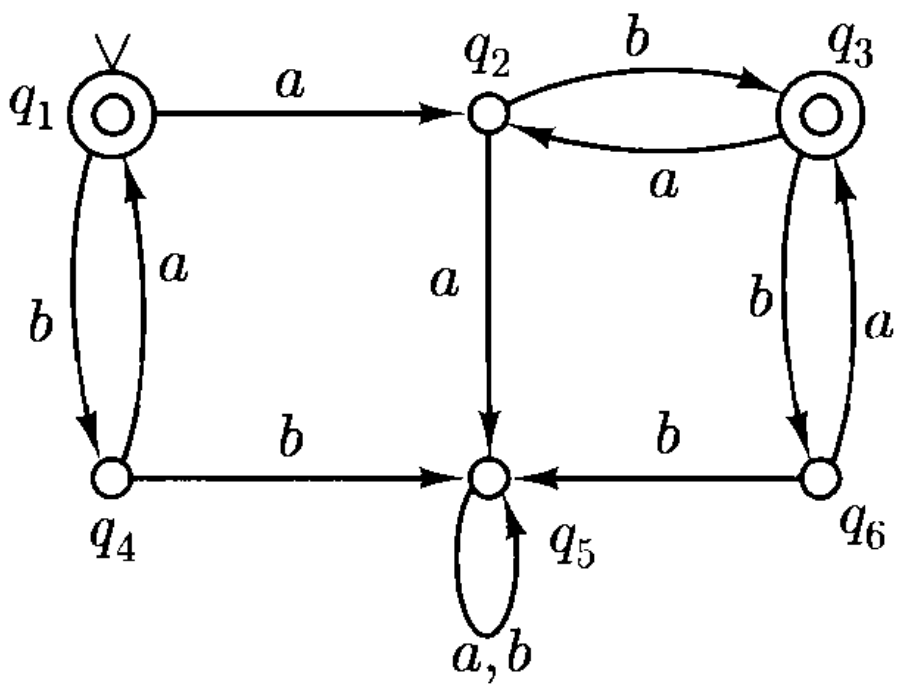
\includegraphics[width=.25\textwidth]{./img/Fig2.20.png}
  \caption{}
\end{figure}

\begin{example}{}
  Let us apply the state minimization algorithm to the deterministic finite automaton $M$ in Figure 19 (same with 17). At the various iterations we shall have these equivalence classes of the corresponding $\equiv_i$:
  \begin{itemize}
    \item Initially, the equivalence classes of $\equiv_{0}$ are $\left\{ q_1, q_3 \right\}$ and $\left\{ q_2, q_4, q_5, q_6 \right\}$.
    \item After the first iteration, the classes of $\equiv_{1}$ are $\left\{ q_1, q_3 \right\}$, $\left\{ q_2 \right\}$, $\left\{ q_4, q_6 \right\}$, and $\left\{ q_5 \right\}$. The splitting happened because $\delta(q_2, b) \not\equiv_{0} \delta(q_4, b), \delta(q_5,b)$, and $\delta(q_4, a) \not\equiv_{0} \delta(q_5,a)$.
    \item After the second iteration, there is no further splitting of classes. The algorithm thus terminates, and the minimum-state automaton is shown in Figure 20. As expected, it is isomorphic with the standard automaton shown in Figure 18.
  \end{itemize}
\end{example}

\begin{figure}[ht]
  \centering
  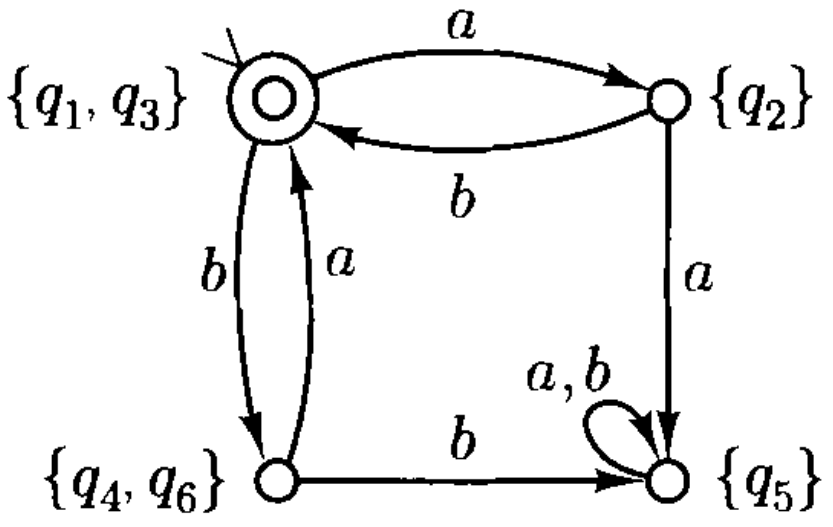
\includegraphics[width=.25\textwidth]{./img/fig2-22.png}
  \caption{}
\end{figure}


% \section{Equivalence Relations and Classes}

\begin{multicols}{2}
\setlength{\columnsep}{1.5cm}
\setlength{\columnseprule}{0.2pt}

\subsection{Equivalence Relations}

In mathematics, an \textbf{\textit{equivalence relation}} is a binary relation that is \textit{reflexive, symmetric} and \textit{transitive}. 

Each equivalence relation provides a partition of the underlying set into disjoint \textit{equivalence classes}. \textit{Two elements of the given set are equivalent to each other if and only if they belong to the same equivalence class.}

\subsubsection{Notation}

Various notations are used in the literature to denote that two elements $a$ and $b$ of a set are equivalent with respect to an equivalence relation $R$; the most common are ``$a \sim b$'' and ``$a \equiv b$'', which are used when $R$ is implicit, and variations of ``$a \sim_{R} b$'', ``$a \equiv_R$'', or ``$a R b$'' to specify $R$ explicitly. Non-equivalence may be written ``$a \not\sim b$'' or ``$a \not\equiv b$''.

\vfill\null
\columnbreak

\subsubsection{Definition}

A binary relation $\sim$ on a set $X$ is said to be an equivalence relation, if and only if it is \textit{reflexive, symmetric} and \textit{transitive}. That is, for all $a, b$, and $c$ in $X$:
\begin{itemize}
    \item $a \sim a$. (Reflexivity)
    \item $a \sim b$ if and only if $b \sim a$. (Symmetry)
    \item If $a \sim b$ and $b \sim c$ then $a \sim c$. (Transitivity)
\end{itemize}
$X$ together with the relation $\sim$ is called a setoid. The equivalence class of $a$ under $\sim$ denoted, $\left[ a \right]$, is defined as $\left[ a \right] = \left\{ x \in X : x \sim a \right\}$

\subsubsection{Example}

On the set $X = \{a,b,c\}$, the relation $R = \{(a, a), (b, b), (c, c), (b, c), (c, b)\}$ is an equivalence relation. The following sets are equivalence classes of this relation:
\begin{multicols}{3}
    \begin{itemize}
        \item $\left[ a \right] = \left\{ a \right\}$
        \item $\left[ b \right] = \left\{ b, c \right\}$
        \item $\left[ c \right] = \left\{ b, c \right\}$
    \end{itemize}
\end{multicols}
\noindent The set of all equivalence classes for $R$ is $\{ \{a\}, \{b,c\} \}$. This set is a partition of the set $X$ with respect to $R$.

\newpage
\subsection{Equivalence Classes}

An \textbf{\textit{equivalence class}} is the name that we give to the subset of $S$ which includes all elements that are equivalent to each other. ``Equivalent'' is dependent on a specified relationship, called an equivalence relation. If there is an equivalence relation between any two elements, they are called equivalent.

Formally, given a set $S$ and an equivalence relation $\sim$, on $S$, the equivalence class of an element $a$ in $S$, denoted by $\left[ a \right]$, is the set

$\begin{aligned}
    \left\{ x \in S : x \sim a \right\}
\end{aligned}$

\noindent of elements which are equivalent to $a$.

\subsubsection{Definition and Notation}

An equivalence relation on a set $X$ is a binary relation $\sim$ on $X$ satisfying the three properties:
\begin{itemize}
    \item $a \sim a$ for all $a \in X$. (Reflexivity)
    \item $a \sim b$ implies $b \sim a$ for all $a, b \in X$. (Symmetry)
    \item If $a \sim b$ and $b \sim c$ then $a \sim c$ for all $a, b, c \in X$. (Transitivity)
\end{itemize}

The equivalence class of an element $a$ is often denoted $\left[ a \right]$ or $\left[ a \right]_{\sim}$ and is defined as the set $\left\{ x \in X : a \sim x \right\}$ of elements that are related to $a$ by $\sim$. The word ``class'' in the term ``equivalence class'' may generally be considered as a synonym of ``set''.

\subsubsection{Properties}

Every element $x$ of $X$ is a member of the equivalence class $\left[ x \right]$. Every two equivalence classes $\left[ a \right]$ and $\left[ b \right]$ are either equal or disjoint. Therefore, the set of all equivalence classes of $X$ forms a partition of $X$: every element of $X$ belongs to one and only one equivalence class. Conversely, every partition of $X$ comes from an equivalence relation in this way, according to which $x \sim y$ if and only if $x$ and $y$ belong to the same set of the partition.

\noindent It follows from the properties of an equivalence relation that

$\begin{aligned}
    x \sim y
\end{aligned}$

\noindent if and only if $\left[ x \right] = \left[ y \right]$.

In other words, if $\sim$ is an equivalence relation on a set $X$, and $x$ and $y$ are two elements of $X$, then these statements are equivalent:
\begin{itemize}
    \item $x \sim y$
    \item $\left[ x \right] = \left[ y \right]$
    \item $\left[ x \right] \cap \left[ y \right] \neq \emptyset$
\end{itemize}

\subsubsection{Examples}

\begin{itemize}
    \item Let $X$ be the set of all rectangles in a plane, and $\sim$ the equivalence relation ``has the same area as'', then for each positive real number $A$, there will be an equivalence class of all the rectangles that have area $A$.
    \item Consider the modulo 2 equivalence relation on the set of integers, $\mathbb{Z}$, such that  $x \sim y$ if and only if their difference $x - y$ is an even number. This relation gives rise to exactly two equivalence classes: One class consists of all even numbers, and the other class consists of all odd numbers. Using square brackets around one member of the class to denote an equivalence class under this relation, $\left[ 7 \right], \left[ 9 \right]$, and $\left[ 1 \right]$ all represent the same element of $\mathbb{Z} / \sim$.
\end{itemize}
\end{multicols}

\end{document}